% 若编译失败,且生成 .synctex(busy) 辅助文件,可能有两个原因:
% 1. 需要插入的图片不存在:Ctrl + F 搜索 'figure' 将这些代码注释/删除掉即可
% 2. 路径/文件名含中文或空格:更改路径/文件名即可

% --------------------- 文章宏包及相关设置 --------------------- %
% >> ------------------ 文章宏包及相关设置 ------------------ << %
% 设定文章类型与编码格式
\documentclass[UTF8]{article}		

% 物理实验报告所需的其它宏包
\usepackage{ulem}   % \uline 下划线支持
\usepackage{circuitikz} % 电路图 tikz 支持
\usepackage{pdfpages}   % 用于导入 pdf 文件

% 本 .tex 专属的宏定义
    \def\V{\ \mathrm{V}}
    \def\uV{\ \mu\mathrm{V}}
    \def\mV{\ \mathrm{mV}}
    \def\K{\ \mathrm{K}}
    \def\kV{\ \mathrm{KV}}
    \def\KV{\ \mathrm{KV}}
    \def\MV{\ \mathrm{MV}}
    \def\uA{\ \mu\mathrm{A}}
    \def\mA{\ \mathrm{mA}}
    \def\A{\ \mathrm{A}}
    \def\kA{\ \mathrm{KA}}
    \def\KA{\ \mathrm{KA}}
    \def\MA{\ \mathrm{MA}}
    \def\O{\ \Omega}
    \def\mO{\ \Omega}
    \def\kO{\ \mathrm{K}\Omega}
    \def\KO{\ \mathrm{K}\Omega}
    \def\MO{\ \mathrm{M}\Omega}
    \def\Hz{\ \mathrm{Hz}}
    \def\uF{\ \mu\mathrm{F}}
    \def\mF{\ \mathrm{mF}}
    \def\F{\ \mathrm{F}}
    \def\Re{\mathrm{\,Re}\,}
    \def\Im{\mathrm{\,Im}\,}
    \def\sinc{\mathrm{\,sinc}\,}

% 自定义宏定义
    \def\N{\mathbb{N}}
    \def\F{\mathbb{F}}
    \def\Z{\mathbb{Z}}
    \def\Q{\mathbb{Q}}
    \def\R{\mathbb{R}}
    \def\C{\mathbb{C}}
    \def\T{\mathbb{T}}
    \def\S{\mathbb{S}}
    %\def\A{\mathbb{A}}
    \def\I{\mathscr{I}}
    \def\d{\mathrm{d}}
    \def\p{\partial}


% 导入基本宏包
    \usepackage[UTF8]{ctex}     % 设置文档为中文语言
    \usepackage{hyperref}  % 宏包:自动生成超链接 (此宏包与标题中的数学环境冲突)
    \hypersetup{
        colorlinks=true,    % false:边框链接 ; true:彩色链接
        citecolor={blue},    % 文献引用颜色
        linkcolor={blue},   % 目录 (我们在目录处单独设置),公式,图表,脚注等内部链接颜色
        urlcolor={magenta},    % 网页 URL 链接颜色,包括 \href 中的 text
        % cyan 浅蓝色 
        % magenta 洋红色
        % yellow 黄色
        % black 黑色
        % white 白色
        % red 红色
        % green 绿色
        % blue 蓝色
        % gray 灰色
        % darkgray 深灰色
        % lightgray 浅灰色
        % brown 棕色
        % lime 石灰色
        % olive 橄榄色
        % orange 橙色
        % pink 粉红色
        % purple 紫色
        % teal 蓝绿色
        % violet 紫罗兰色
    }
    % \usepackage{docmute}    % 宏包:子文件导入时自动去除导言区,用于主/子文件的写作方式,\include{./51单片机笔记}即可。注:启用此宏包会导致.tex文件capacity受限。
    \usepackage{amsmath}    % 宏包:数学公式
    \usepackage{mathrsfs}   % 宏包:提供更多数学符号
    \usepackage{amssymb}    % 宏包:提供更多数学符号
    \usepackage{pifont}     % 宏包:提供了特殊符号和字体
    \usepackage{extarrows}  % 宏包:更多箭头符号 
    \usepackage{multicol}   % 宏包:支持多栏 

% 文章页面margin设置
    \usepackage[a4paper]{geometry}
        \geometry{top=0.75in}
        \geometry{bottom=0.75in}
        \geometry{left=0.75in}
        \geometry{right=0.75in}   % 设置上下左右页边距
        \geometry{marginparwidth=1.75cm}    % 设置边注距离(注释、标记等)

% 配置数学环境
    \usepackage{amsthm} % 宏包:数学环境配置
    % theorem-line 环境自定义
        \newtheoremstyle{MyLineTheoremStyle}% <name>
            {11pt}% <space above>
            {11pt}% <space below>
            {\kaishu}% <body font> 默认使用正文字体, \kaishu 为楷体
            {}% <indent amount>
            {\bfseries}% <theorem head font> 设置标题项为加粗
            {:\ \ }% <punctuation after theorem head>
            {.5em}% <space after theorem head>
            {\textbf{#1}\thmnumber{#2}\ \ (\,\textbf{#3}\,)}% 设置标题内容顺序
        \theoremstyle{MyLineTheoremStyle} % 应用自定义的定理样式
        \newtheorem{LineTheorem}{Theorem.\,}
    % theorem-block 环境自定义
        \newtheoremstyle{MyBlockTheoremStyle}% <name>
            {11pt}% <space above>
            {11pt}% <space below>
            {\kaishu}% <body font> 使用默认正文字体
            {}% <indent amount>
            {\bfseries}% <theorem head font> 设置标题项为加粗
            {:\\ \indent}% <punctuation after theorem head>
            {.5em}% <space after theorem head>
            {\textbf{#1}\thmnumber{#2}\ \ (\,\textbf{#3}\,)}% 设置标题内容顺序
        \theoremstyle{MyBlockTheoremStyle} % 应用自定义的定理样式
        \newtheorem{BlockTheorem}[LineTheorem]{Theorem.\,} % 使用 LineTheorem 的计数器
    % definition 环境自定义
        \newtheoremstyle{MySubsubsectionStyle}% <name>
            {11pt}% <space above>
            {11pt}% <space below>
            {}% <body font> 使用默认正文字体
            {}% <indent amount>
            {\bfseries}% <theorem head font> 设置标题项为加粗
            {:\\ \indent}% <punctuation after theorem head>
            {0pt}% <space after theorem head>
            {\textbf{#3}}% 设置标题内容顺序
        \theoremstyle{MySubsubsectionStyle} % 应用自定义的定理样式
        \newtheorem{definition}{}

%宏包:有色文本框(proof环境)及其设置
\usepackage{xcolor}    %设置插入的文本框颜色
    % rgb(4, 9, 103), rgb(5, 13, 164)
    % rgb(124, 131, 255), rgb(231, 232, 255)
    % rgb(255, 190, 190), rgb(255, 70, 70)
    \definecolor{stc}{RGB}{4, 10, 118}  % 设置各级标题结构颜色
\usepackage[strict]{changepage}     % 提供一个 adjustwidth 环境
\usepackage{framed}     % 实现方框效果
    % rgb(0, 0, 0), rgb(100, 100, 100)
    %#ECECED 为 0.93, 0.93, 0.93
    \definecolor{graybox_color}{rgb}{0.93, 0.93, 0.93} % 这里的 rbg 范围是 [0, 1]
    % 文本框颜色。修改此行中的 rgb 数值即可改变方框纹颜色,具体颜色的rgb数值可以在网站https://colordrop.io/ 中获得。(截止目前的尝试还没有成功过,感觉单位不一样)(找到喜欢的颜色,点击下方的小眼睛,找到rgb值,复制修改即可)
    \newenvironment{graybox}{%
    \def\FrameCommand{%
    \hspace{1pt}%
    {\color{gray}\small \vrule width 2pt}%
    {\color{graybox_color}\vrule width 4pt}%
    \colorbox{graybox_color}%
    }%
    \MakeFramed{\advance\hsize-\width\FrameRestore}%
    \noindent\hspace{-4.55pt}% disable indenting first paragraph
    \begin{adjustwidth}{}{7pt}%
    \vspace{2pt}\vspace{2pt}%
    }
    {%
    \vspace{2pt}\end{adjustwidth}\endMakeFramed%
    }

    \definecolor{bluebox_ruleColor}{rgb}{0.49, 0.51, 1} % 文本框颜色。修改此行中的 rgb 数值即可改变方框纹颜色,具体颜色的rgb数值可以在网站https://colordrop.io/ 中获得。(截止目前的尝试还没有成功过,感觉单位不一样)(找到喜欢的颜色,点击下方的小眼睛,找到rgb值,复制修改即可)
    \definecolor{bluebox_backgroundColor}{rgb}{0.93, 0.93, 1}
    \newenvironment{bluebox}{%
    \def\FrameCommand{%
    \hspace{1pt}%
    {\color{bluebox_ruleColor}\small \vrule width 2pt}%
    {\color{bluebox_backgroundColor}\vrule width 4pt}% 4pt 缩进比较合适
    \colorbox{bluebox_backgroundColor}%
    }%
    \MakeFramed{\advance\hsize-\width\FrameRestore}%
    \noindent\hspace{-4.55pt}% disable indenting first paragraph
    \begin{adjustwidth}{}{7pt}%
    \vspace{2pt}\vspace{2pt}%
    }
    {%
    \vspace{2pt}\end{adjustwidth}\endMakeFramed%
    }

    \definecolor{redbox_ruleColor}{rgb}{1, 0.27, 0.27} % 文本框颜色。修改此行中的 rgb 数值即可改变方框纹颜色,具体颜色的rgb数值可以在网站https://colordrop.io/ 中获得。(截止目前的尝试还没有成功过,感觉单位不一样)(找到喜欢的颜色,点击下方的小眼睛,找到rgb值,复制修改即可)
    \definecolor{redbox_backgroundColor}{rgb}{1, 0.90, 0.90}
    \newenvironment{redbox}{%
    \def\FrameCommand{%
    \hspace{1pt}%
    {\color{redbox_ruleColor}\small \vrule width 2pt}%
    {\color{redbox_backgroundColor}\vrule width 4pt}% 4pt 缩进比较合适
    \colorbox{redbox_backgroundColor}%
    }%
    \MakeFramed{\advance\hsize-\width\FrameRestore}%
    \noindent\hspace{-4.55pt}% disable indenting first paragraph
    \begin{adjustwidth}{}{7pt}%
    \vspace{2pt}\vspace{2pt}%
    }
    {%
    \vspace{2pt}\end{adjustwidth}\endMakeFramed%
    }

% 外源代码插入设置
    % matlab 代码插入设置
    \usepackage{matlab-prettifier}
        \lstset{style=Matlab-editor}    % 继承 matlab 代码高亮 , 此行不能删去
    \usepackage[most]{tcolorbox} % 引入tcolorbox包 
    \usepackage{listings} % 引入listings包
        \tcbuselibrary{listings, skins, breakable}
        \newfontfamily\codefont{Consolas} % 定义需要的 codefont 字体
        \lstdefinestyle{MatlabStyle_inc}{   % 插入代码的样式
            language=Matlab,
            basicstyle=\footnotesize\ttfamily\codefont,    % ttfamily 确保等宽 
            breakatwhitespace=false,
            breaklines=true,
            captionpos=b,
            keepspaces=true,
            numbers=left,
            numbersep=15pt,
            showspaces=false,
            showstringspaces=false,
            showtabs=false,
            tabsize=2,
            xleftmargin=15pt,   % 左边距
            %frame=single, % single 为包围式单线框
            frame=shadowbox,    % shadowbox 为带阴影包围式单线框效果
            %escapeinside=``,   % 允许在代码块中使用 LaTeX 命令 (此行无用)
            %frameround=tttt,    % tttt 表示四个角都是圆角
            framextopmargin=0pt,    % 边框上边距
            framexbottommargin=0pt, % 边框下边距
            framexleftmargin=5pt,   % 边框左边距
            framexrightmargin=5pt,  % 边框右边距
            rulesepcolor=\color{red!20!green!20!blue!20}, % 阴影框颜色设置
            %backgroundcolor=\color{blue!10}, % 背景颜色
        }
        \lstdefinestyle{MatlabStyle_src}{   % 插入代码的样式
            language=Matlab,
            basicstyle=\small\ttfamily\codefont,    % ttfamily 确保等宽 
            breakatwhitespace=false,
            breaklines=true,
            captionpos=b,
            keepspaces=true,
            numbers=left,
            numbersep=15pt,
            showspaces=false,
            showstringspaces=false,
            showtabs=false,
            tabsize=2,
        }
        \newtcblisting{matlablisting}{
            %arc=2pt,        % 圆角半径
            % 调整代码在 listing 中的位置以和引入文件时的格式相同
            top=0pt,
            bottom=0pt,
            left=-5pt,
            right=-5pt,
            listing only,   % 此句不能删去
            listing style=MatlabStyle_src,
            breakable,
            colback=white,   % 选一个合适的颜色
            colframe=black!0,   % 感叹号后跟不透明度 (为 0 时完全透明)
        }
        \lstset{
            style=MatlabStyle_inc,
        }

% table 支持
    \usepackage{booktabs}   % 宏包:三线表
    \usepackage{tabularray} % 宏包:表格排版
    \usepackage{longtable}  % 宏包:长表格

% figure 设置
    \usepackage{graphicx}  % 支持 jpg, png, eps, pdf 图片 
    \usepackage{svg}       % 支持 svg 图片
        \svgsetup{
            % 指向 inkscape.exe 的路径
            inkscapeexe = C:/aa_MySame/inkscape/bin/inkscape.exe, 
            % 一定程度上修复导入后图片文字溢出几何图形的问题
            inkscapelatex = false                 
        }
    \usepackage{subcaption} % 用于子图和小图注  

% 图表进阶设置
    \usepackage{caption}    % 图注、表注
        \captionsetup[figure]{name=图}  
        \captionsetup[table]{name=表}
        \captionsetup{
            labelfont=bf, % 设置标签为粗体
            textfont=bf,  % 设置文本为粗体
            font=small  
        }
    \usepackage{float}     % 图表位置浮动设置 
    \usepackage{etoolbox} % 用于保证图注表注的数学字符为粗体
        \AtBeginEnvironment{figure}{\boldmath} % 图注中的数学字符为粗体
        \AtBeginEnvironment{table}{\boldmath}  % 表注中的数学字符为粗体
        \AtBeginEnvironment{tabular}{\unboldmath}   % 保证表格中的数学字符不受额外影响

% 圆圈序号自定义
    \newcommand*\circled[1]{\tikz[baseline=(char.base)]{\node[shape=circle,draw,inner sep=0.8pt, line width = 0.03em] (char) {\bfseries #1};}}   % TikZ solution

% 列表设置
    \usepackage{enumitem}   % 宏包:列表环境设置
        \setlist[enumerate]{
            label=(\arabic*) ,   % 设置序号样式为加粗的 (1) (2) (3)
            ref=\arabic*, % 如果需要引用列表项,这将决定引用格式(这里仍然使用数字)
            itemsep=0pt, parsep=0pt, topsep=0pt, partopsep=0pt, leftmargin=3.5em} 
        \setlist[itemize]{itemsep=0pt, parsep=0pt, topsep=0pt, partopsep=0pt, leftmargin=3.5em}
        \newlist{circledenum}{enumerate}{1} % 创建一个新的枚举环境  
        \setlist[circledenum,1]{  
            label=\protect\circled{\arabic*}, % 使用 \arabic* 来获取当前枚举计数器的值,并用 \circled 包装它  
            ref=\arabic*, % 如果需要引用列表项,这将决定引用格式(这里仍然使用数字)
            itemsep=0pt, parsep=0pt, topsep=0pt, partopsep=0pt, leftmargin=3.5em
        }  

% 其它设置
    % 脚注设置
        \renewcommand\thefootnote{\ding{\numexpr171+\value{footnote}}}
    % 参考文献引用设置
        \bibliographystyle{unsrt}   % 设置参考文献引用格式为unsrt
        \newcommand{\upcite}[1]{\textsuperscript{\cite{#1}}}     % 自定义上角标式引用
    % 文章序言设置
        \newcommand{\cnabstractname}{序言}
        \newenvironment{cnabstract}{%
            \par\Large
            \noindent\mbox{}\hfill{\bfseries \cnabstractname}\hfill\mbox{}\par
            \vskip 2.5ex
            }{\par\vskip 2.5ex}

% 文章默认字体设置
    \usepackage{fontspec}   % 宏包:字体设置
        \setmainfont{SimSun}    % 设置中文字体为宋体字体
        \setCJKmainfont[AutoFakeBold=3]{SimSun} % 设置加粗字体为 SimSun 族,AutoFakeBold 可以调整字体粗细
        \setmainfont{Times New Roman} % 设置英文字体为Times New Roman

% 各级标题自定义设置
    \usepackage{titlesec}   
        % section标题自定义设置 
        \titleformat{\section}[hang]{\normalfont\Large\bfseries\boldmath}{\thesection}{8pt}{}
        % subsection 标题自定义设置
        \titleformat{\subsection}[hang]{\normalfont\large\bfseries\boldmath}{\thesubsection}{8pt}{}
        \titlespacing*{\subsection}{0pt}{10pt}{6pt} % 控制上下间距


% --------------------- 文章宏包及相关设置 --------------------- %
% >> ------------------ 文章宏包及相关设置 ------------------ << %




% ------------------------ 文章信息区 ------------------------ %
% ------------------------ 文章信息区 ------------------------ %
% 页眉页脚设置
\usepackage{fancyhdr}   %宏包:页眉页脚设置
    \pagestyle{fancy}
    \fancyhf{}
    \cfoot{\thepage}
    \renewcommand\headrulewidth{1pt}
    \renewcommand\footrulewidth{0pt}
    %\rhead{《线性电路实验》实验报告}    
    \lhead{\small \faGithub\ \href{https://github.com/YiDingg/UCAS-LinearCircuitExperiment}{\color{black} https://github.com/YiDingg/UCAS-LinearCircuitExperiment}}


    \graphicspath{{../}}   % 修改主文件图像路径,使得子文件能够直接使用相对路径,而不是从 assets 开始索引

    \usepackage{fontawesome}    % 宏包:更多符号与图标 (用于插入 GitHub 图标等)



%%%%%%%%%%%%%%%%%%%%%%%%%%%%%%%%%%%%%%%%%%%%%%%%%%%%%%%%%%%%%%%%
% 仅需修改页眉、实验名称、实验日期
%%%%%%%%%%%%%%%%%%%%%%%%%%%%%%%%%%%%%%%%%%%%%%%%%%%%%%%%%%%%%%%%


%%%%%%%%%%%%%%%%%% 1. 修改页眉内容 %%%%%%%%%%%%%%%%%%
\rhead{LCE-02 三极管 (2025.04.11, 丁毅)}


% 开始编辑文章
\begin{document}
\begin{center}\large
    \vspace*{-0.8cm}
    \noindent{\huge\bfseries《\ \ 线\ \ 性\ \ 电\ \ 路\ \ 实\ \ 验\ \ \ 》\ \ 实\ \ 验\ \ 报\ \ 告 }
    \\\vspace{0.1cm}
    \noindent{
    {\bfseries 
%
%%%%%%%%%%%%%%%%%% 2. 修改实验名称 %%%%%%%%%%%%%%%%%%
    实验名称:\uline{\hspace{2.2cm} 三极管 \hspace{2.2cm}}
%%%%%%%%%%%%%%%%%% 2. 修改实验名称 %%%%%%%%%%%%%%%%%%
%
    }\hspace{0.4cm}
    指导教师:\uline{\hspace{0.8cm}王东雷\ \ \ \  \ df4dac@sina.com     \hspace{0.8cm}}
    }
    \\\vspace{0.1cm}
    \noindent
    {
    姓名:\uline{\,\,\,丁毅\,\,\,}\hspace{0.2cm}
    学号:\uline{\,\,\,{ 2023K8009908031}\,\,\,}\hspace{0.2cm}
    班级/专业:\uline{\,\,\,{2308/电子信息}\,\,\,}\hspace{0.2cm}
    分组序号:\uline{\,\,\,{2-06}\,\,\,}
    }
    \\\vspace{0.1cm}
    \noindent{
%
%%%%%%%%%%%%%%%%%% 3. 修改实验日期 %%%%%%%%%%%%%%%%%%
    实验日期:\uline{\,\,{2025.04.11}\,\,}\hspace{0.2cm}
%%%%%%%%%%%%%%%%%% 3. 修改实验日期 %%%%%%%%%%%%%%%%%%
%
    实验地点:\uline{\,\,\,教学楼{ 607}\,\,\,}\hspace{0.2cm}
    是否调课/补课:\uline{\hspace{0.26cm}否 \hspace{0.26cm}}\hspace{0.2cm}
    成绩:\uline{\hspace{2cm}}
    }
\end{center}
\vspace{-0.4cm}
\noindent\rule{\textwidth}{0.075em}   % 分割线
\vspace{-1.0cm}

% 生成目录
\setcounter{tocdepth}{3}  % 目录深度为 2(不显示 subsubsection)
\noindent\tableofcontents\thispagestyle{fancy}   % 显示页码、页眉等

% ------------------------ 文章信息区 ------------------------ %
% ------------------------ 文章信息区 ------------------------ %



%%%%%%%%%%%%%%%%%%%%%%%%%%%%%%%%%%%%%%%%%%%%%%%%%%%%%%%%%%%%%%%%%%%%%%%%%%%%%%%%%
%%%%%%%%%%%%%%%%%%%%%%%%%%%%%%%%% 下面是正文内容 %%%%%%%%%%%%%%%%%%%%%%%%%%%%%%%%%
%%%%%%%%%%%%%%%%%%%%%%%%%%%%%%%%%%%%%%%%%%%%%%%%%%%%%%%%%%%%%%%%%%%%%%%%%%%%%%%%%

\newpage
\section{实验目的}

\begin{enumerate}
    \item 进一步认识三极管,加深对三极管放大电路的理解;
    \item 进一步熟悉信号源与示波器,掌握示波器扫频 (Sweep) 测试方法;
    \item 简单焊接练习;
    \item 观察双极性晶体管开关波形。
\end{enumerate}


\section{实验仪器}

\begin{enumerate}
    \item 数字万用表: Unit UT61E (C190241394)
    \item 数字示波器: RIGOL 200MSO2202A (DS2F192200361)
    \item 信号发生器: Goodwill AFG-22225 (GER910370)
    \item 数字直流电源: GWINSTEK GPD-3303S (GES813705)
    \item 其它:双极型晶体管 BC547C、S8050;电解电容、陶瓷电容、电位器、电阻、跳线、PCB 测试点
\end{enumerate}

\section{实验内容及实验结果}

\subsection{用万用表简单测量三极管是否损坏}

使用万用表二极管挡测量,由于三极管 BE, BC 可以分别视为 PN 结,故可以利用万
用表二极管档测量每个 PN 结的导通压降来简单判断各引脚、管内部是否损坏(正常情况下示数
应为 0.7 V 左右)。下表是测量数据和判断结果:

\begin{table}[H]\centering
    %\renewcommand{\arraystretch}{1.5} % 调整行间距
    %\setlength{\tabcolsep}{1.5mm} % 调整列间距
    \caption{三极管引脚测量结果}
    \label{三极管引脚测量结果}
\begin{tabular}{cccccccccc}\toprule
    型号 & $V_{BE}$ (V) & $V_{BC}$ (V) & $V_{D}$ (V)  \\
    \midrule
    BC547C & 0.6996 & 0.6971 & 0.6198 \\
    S8050  & 0.6974 & 0.7006 & 0.5970 \\
    3DG12C & 0.6826 & 0.6788 & 0.6153 \\
    \bottomrule
\end{tabular}
\end{table}
\noindent 其中 $V_D$ 是将 BC 短接,测量 B 与 E 之间的压降,也就是 ``diode-connected" 连接。


\subsection{共射放大电路 (Common-Emitter Amplifier)}
\vspace*{-4mm}
\begin{redbox}
若无特别说明,本小节的输入信号默认为 1 kHz sine wave, 示波器耦合为 ac coupling 。
\end{redbox}

\subsubsection{直流工作点}

按预习报告中的电路图正确连接电路,然后使用万用表测量直流工作点,结果如下;

\begin{center}
\noindent\begin{minipage}{0.74\columnwidth}
    \begin{figure}[H]\centering
        \begin{subfigure}[b]{0.5\columnwidth}\centering
            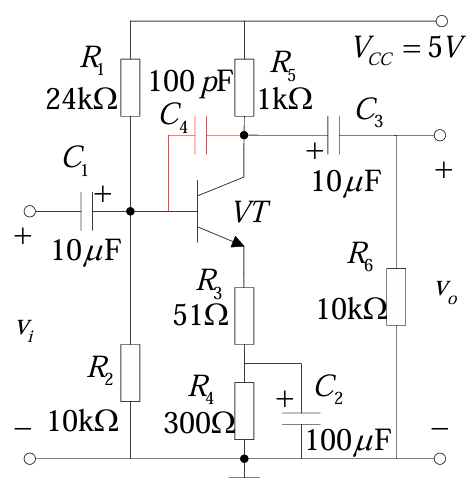
\includegraphics[height=150pt]{preview/assets/CE.png}
            \caption{Circuit Schematic}
        \end{subfigure}\hfill
        \begin{subfigure}[b]{0.5\columnwidth}\centering
            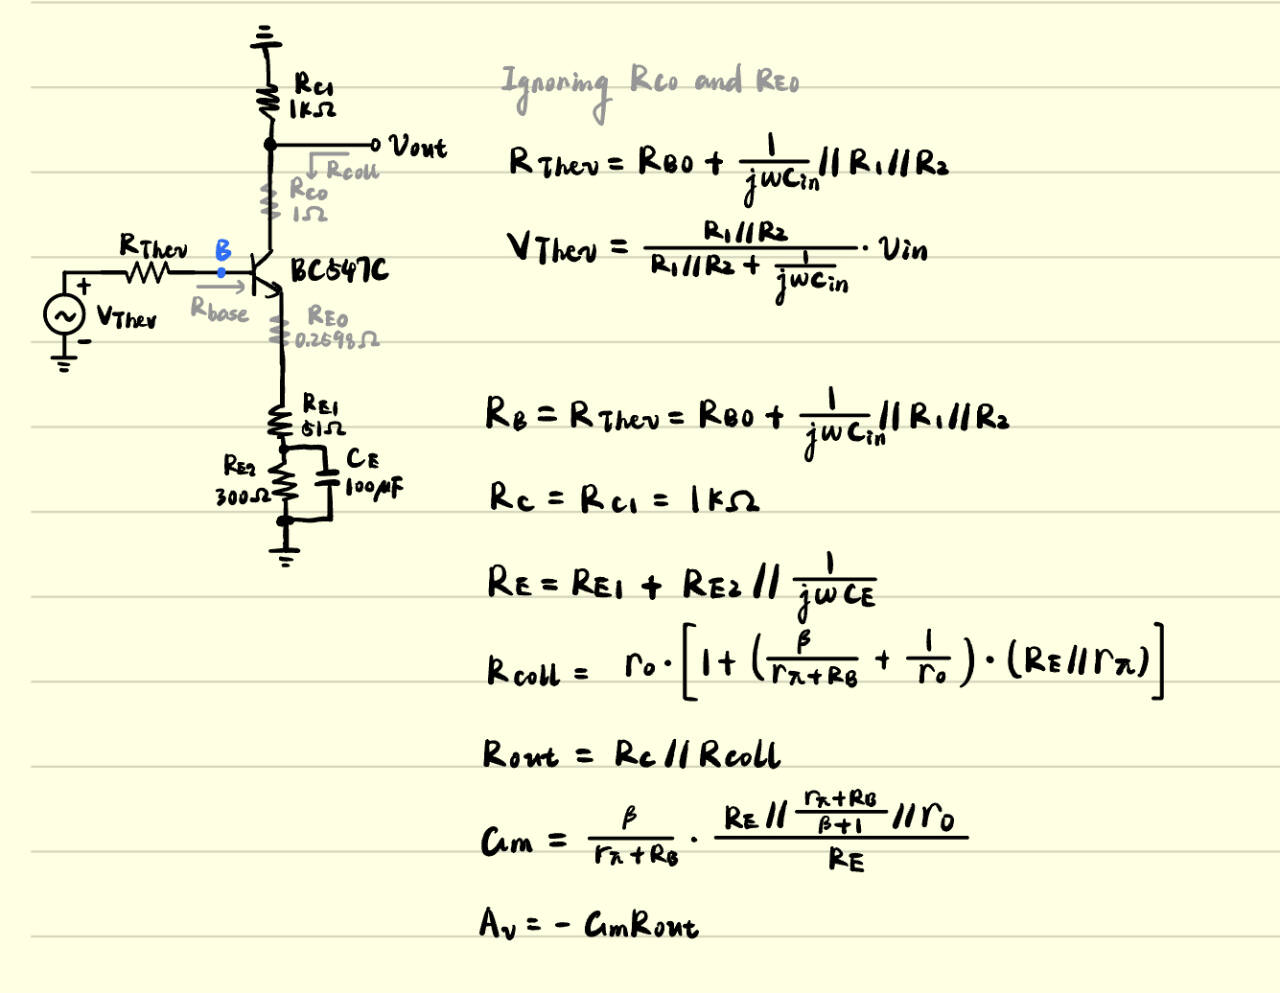
\includegraphics[height=140pt]{preview/assets/Gain.png}
            \caption{Small-Signal (Mid-band) Gain Calculation}
        \end{subfigure}
        \caption{Design of Common-Emitter Amplifier}
    \end{figure}
\end{minipage}\hfill\begin{minipage}{0.25\columnwidth}
    \begin{gather}
        V_{CC} = 5 \ \mathrm{V}\\
        I_C = 2.303\ \mathrm{mA}    \\
        V_{CE} = 1.8780\ \mathrm{V}  \\
        V_{BE} = 0.6326\ \mathrm{V}
    \end{gather}
\end{minipage}\end{center}

\subsubsection{中频小信号增益}

为获得较准确的小信号增益,输入信号应足够小。令信号源输入电阻 $R_S = 0 $, 负载电阻 $R_L = \infty$,分别设置输入信号幅度为 20 mVamp, 50 mVamp, 测量输出波形,结果如下:

\begin{figure}[H]\centering
    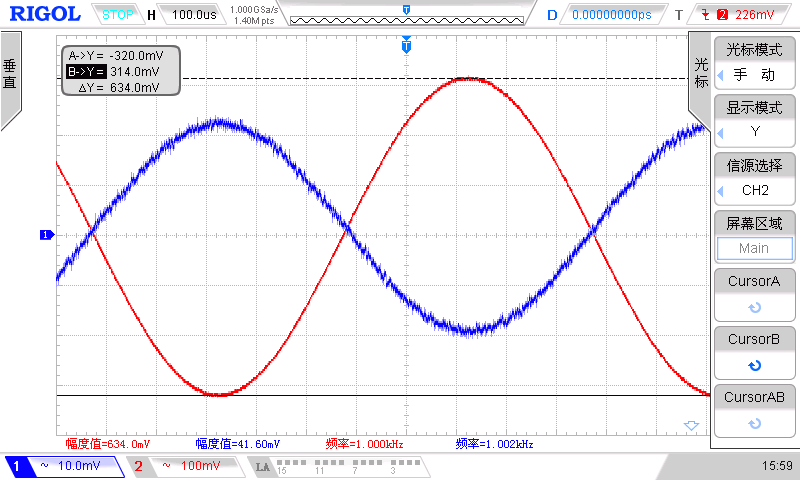
\includegraphics[width=\columnwidth]{LCE-02-三极管/assets/原始增益 input 20 mVamp (40 mVpp), R_S = 0, R_L = inf.png}
    \caption{CE amplifier I/O curve: ac coupling, input 20 mVamp, 有效输入 $V_{B}$ (CH1, blue),输出电压 $V_{out}$ (CH2, red)}
\end{figure}
\begin{figure}[H]\centering
    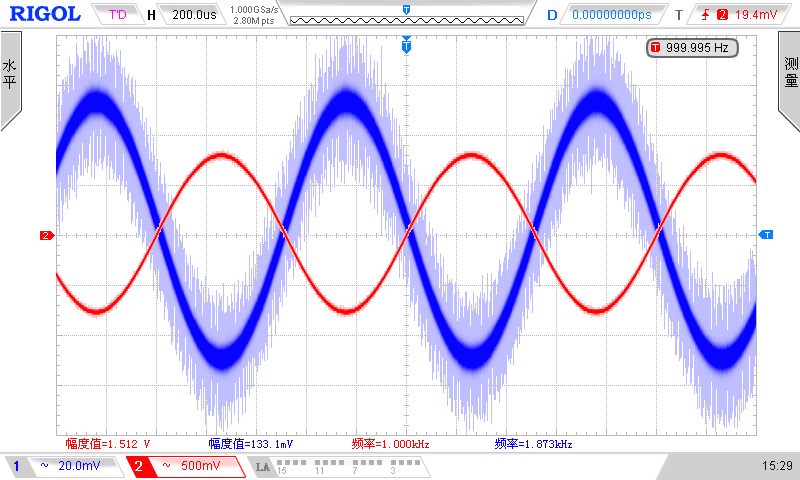
\includegraphics[width=\columnwidth]{LCE-02-三极管/assets/CE input 50mVamp (R_S = 0), 正常线性放大.png}
    \caption{CE amplifier I/O curve: ac coupling, input 50 mVamp, 有效输入 $V_{B}$ (CH1, blue),输出电压 $V_{out}$ (CH2, red), 错位显示}
\end{figure}
\begin{figure}[H]\centering
    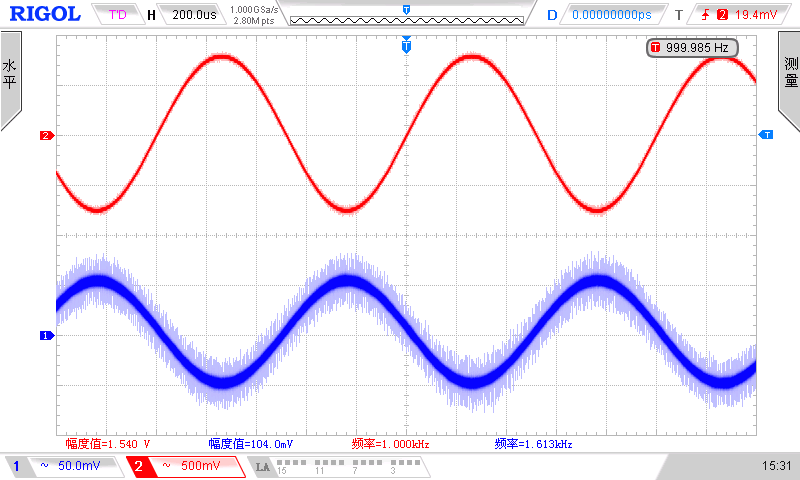
\includegraphics[width=\columnwidth]{LCE-02-三极管/assets/CE input 50mVamp (R_S = 0), 正常线性放大 错位显示.png}
    \caption{CE amplifier I/O curve: ac coupling, input 50 mVamp, 有效输入 $V_{B}$ (CH1, blue),输出电压 $V_{out}$ (CH2, red), 错位显示}
\end{figure}



利用输入 20 mVamp 时所得的结果,计算中频小信号增益:
\begin{gather}
|A_0| = |A_{v, 1\ \mathrm{kHz}}| = \frac{V_{out,pp}}{V_{in,pp}} = \frac{634 \ \mathrm{mV}}{40 \ \mathrm{mV}} = 15.85 
\end{gather}


\subsubsection{饱和与截止失真}

当输入信号的幅度过大(等价于输出信号幅度过大)时,会出现饱和失真和截止失真。其中,饱和失真更明显,容易识别,截止失真是非线性失真的典例,肉眼通常无法准确识别。设置输入信号为 150 mVamp, 得到输出曲线如下:

\begin{figure}[H]\centering
    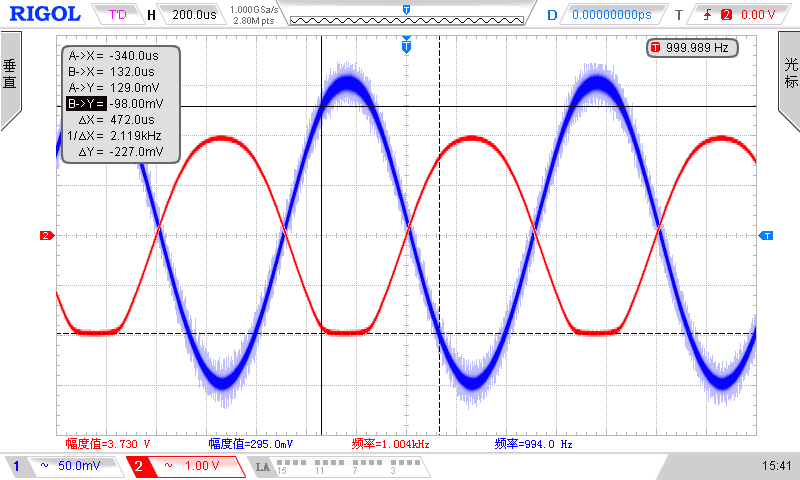
\includegraphics[width=\columnwidth]{LCE-02-三极管/assets/CE 截止与饱和失真 - Vin 范围, input 150 mVamp.png}
    \caption{CE amplifier I/O curve: input 150 mVamp, 有效输入 $V_{B}$ (CH1, blue),输出电压 $V_{out}$ (CH2, red),测量输入信号范围}
\end{figure}
\begin{figure}[H]\centering
    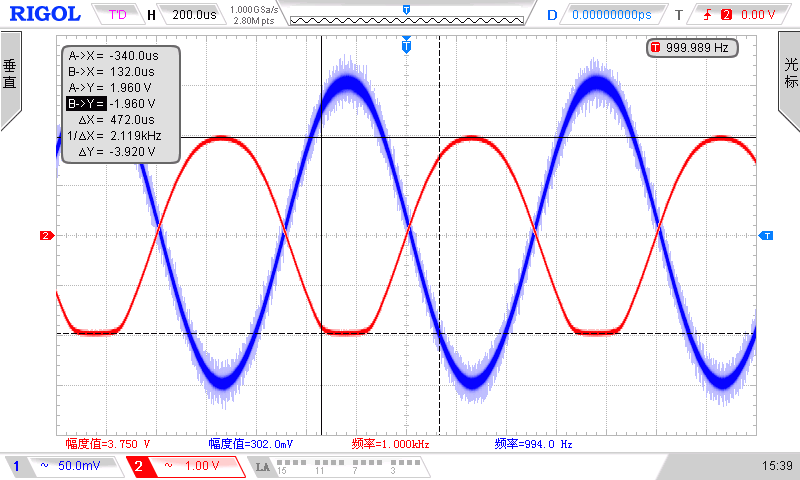
\includegraphics[width=\columnwidth]{LCE-02-三极管/assets/CE 截止与饱和失真 - Vout 范围, input 150 mVamp.png}
    \caption{CE amplifier I/O curve: input 150 mVamp, 有效输入 $V_{B}$ (CH1, blue),输出电压 $V_{out}$ (CH2, red),测量输出信号范围}
\end{figure}
\begin{figure}[H]\centering
    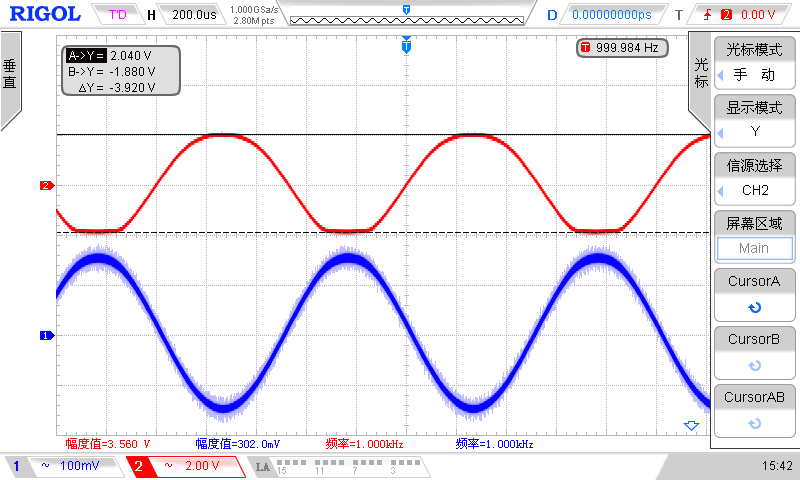
\includegraphics[width=\columnwidth]{LCE-02-三极管/assets/CE 截止与饱和失真 (错位) - Vout 范围, input 150 mVamp.png}
    \caption{CE amplifier I/O curve: input 150 mVamp, 有效输入 $V_{B}$ (CH1, blue),输出电压 $V_{out}$ (CH2, red),测量输出信号范围}
\end{figure}

在上面三个图中,饱和失真出现在 $V_{in}$ 高、$V_{out}$ 低的位置,而截止失真出现在 $V_{in}$ 低、$V_{out}$ 高的位置。由图可以看出,为避免出现饱和失真和截止失真,输入输出交流信号范围分别约为:
\begin{gather}
V_{in} \in (-100 \ \mathrm{mV},\ 129 \ \mathrm{mV}),\quad 
V_{out} \in (-2 \ \mathrm{V},\ 1.677 \ \mathrm{V}),\quad 
(V_{out,pp})_{\max} = 1.677 \ \mathrm{V} - (-2 \ \mathrm{V}) = 3.677 \ \mathrm{V}
\end{gather}

\noindent 如果要避免出现饱和失真,但是可以忍受一定的截止失真,则输出交流信号大约被限制在:
\begin{gather}
V_{out} \in (-2 \ \mathrm{V},\ 2 \ \mathrm{V}),\quad 
(V_{out,pp})_{\max} = 2 \ \mathrm{V} - (-2 \ \mathrm{V}) = 4 \ \mathrm{V}
\end{gather}



\subsubsection{输入输出阻抗}

利用输入(或输出)等效戴维南电路的分压,测量输出端小信号增益的变化,可以计算输入输出阻抗。我们先测量 $R_S = 1\ \mathrm{k}\Omega,\ R_L = \infty$ 的小信号增益,再测量 $R_S = 0,\ R_L = 2\ \mathrm{k}\Omega$ 的增益,结果如下:
\begin{figure}[H]\centering
    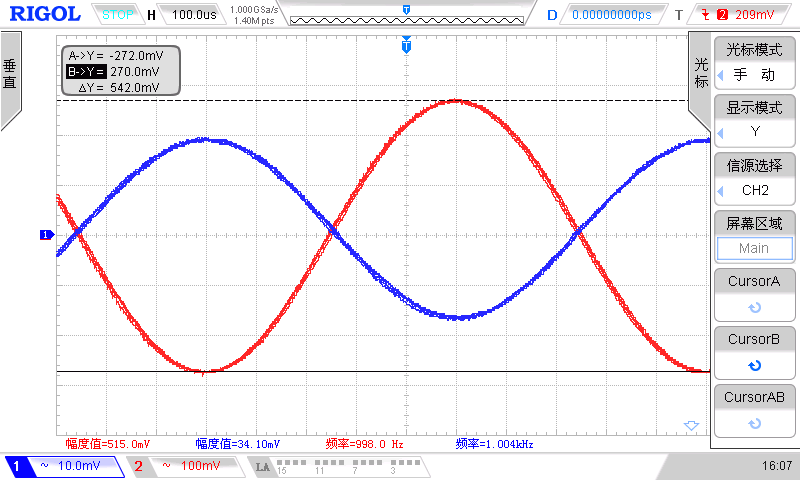
\includegraphics[width=\columnwidth]{LCE-02-三极管/assets/输入阻抗 R_S = 1k.png}
    \caption{Input impedance: input 20 mVamp, $(R_S, R_L) = (1 \ \mathrm{k}\Omega, \infty)$, 有效输入 $V_{B}$ (CH1, blue),输出电压 $V_{out}$ (CH2, red)}
    \label{fig: Input impedance}
\end{figure}
\begin{figure}[H]\centering
    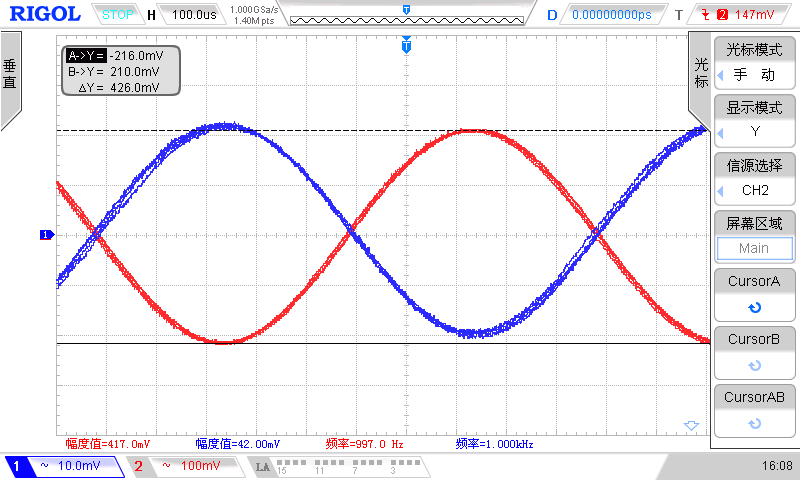
\includegraphics[width=\columnwidth]{LCE-02-三极管/assets/输出阻抗 R_L = 2k.png}
    \caption{Output impedance: input 20 mVamp, $(R_S, R_L) = (0, 2 \ \mathrm{k}\Omega)$, 有效输入 $V_{B}$ (CH1, blue),输出电压 $V_{out}$ (CH2, red)}
    \label{fig: Output impedance}
\end{figure}

分别计算输入、输出阻抗:
\begin{gather}
\mathrm{Input\ impedance: \ \ } V_{out,pp}' = 542 \ \mathrm{mV}
\Longrightarrow 
R_{in} = \frac{R_S}{\frac{V_{out,pp}}{V_{out,pp}'} - 1} 
= \frac{1 \ \mathrm{k}\Omega}{\frac{634 \ \mathrm{mV}}{542 \ \mathrm{mV}} - 1}
= 5.8913 \ \mathrm{k}\Omega
\\ 
\mathrm{Output\ impedance: \ \ } V_{out,pp}' = 426 \ \mathrm{mV}
\Longrightarrow 
R_{out} = \left(\frac{V_{out,pp}}{V_{out,pp}'} - 1\right) R_L 
= 0.9765 \ \mathrm{k}\Omega
\end{gather}

而 1 kHz 处的理论计算值(见图 \ref{fig: Input and output impedance theoretical results})为 $R_{in} = 5.571 \ \mathrm{k}\Omega$, $R_{out} = 1.007 \ \mathrm{k}\Omega$,与我们的实测值基本吻合。理论推导过程详见\textbf{附录 C (Experiment Report of Common Emitter Amplifier)},我们这里不多赘述。

\begin{figure}[H]\centering
    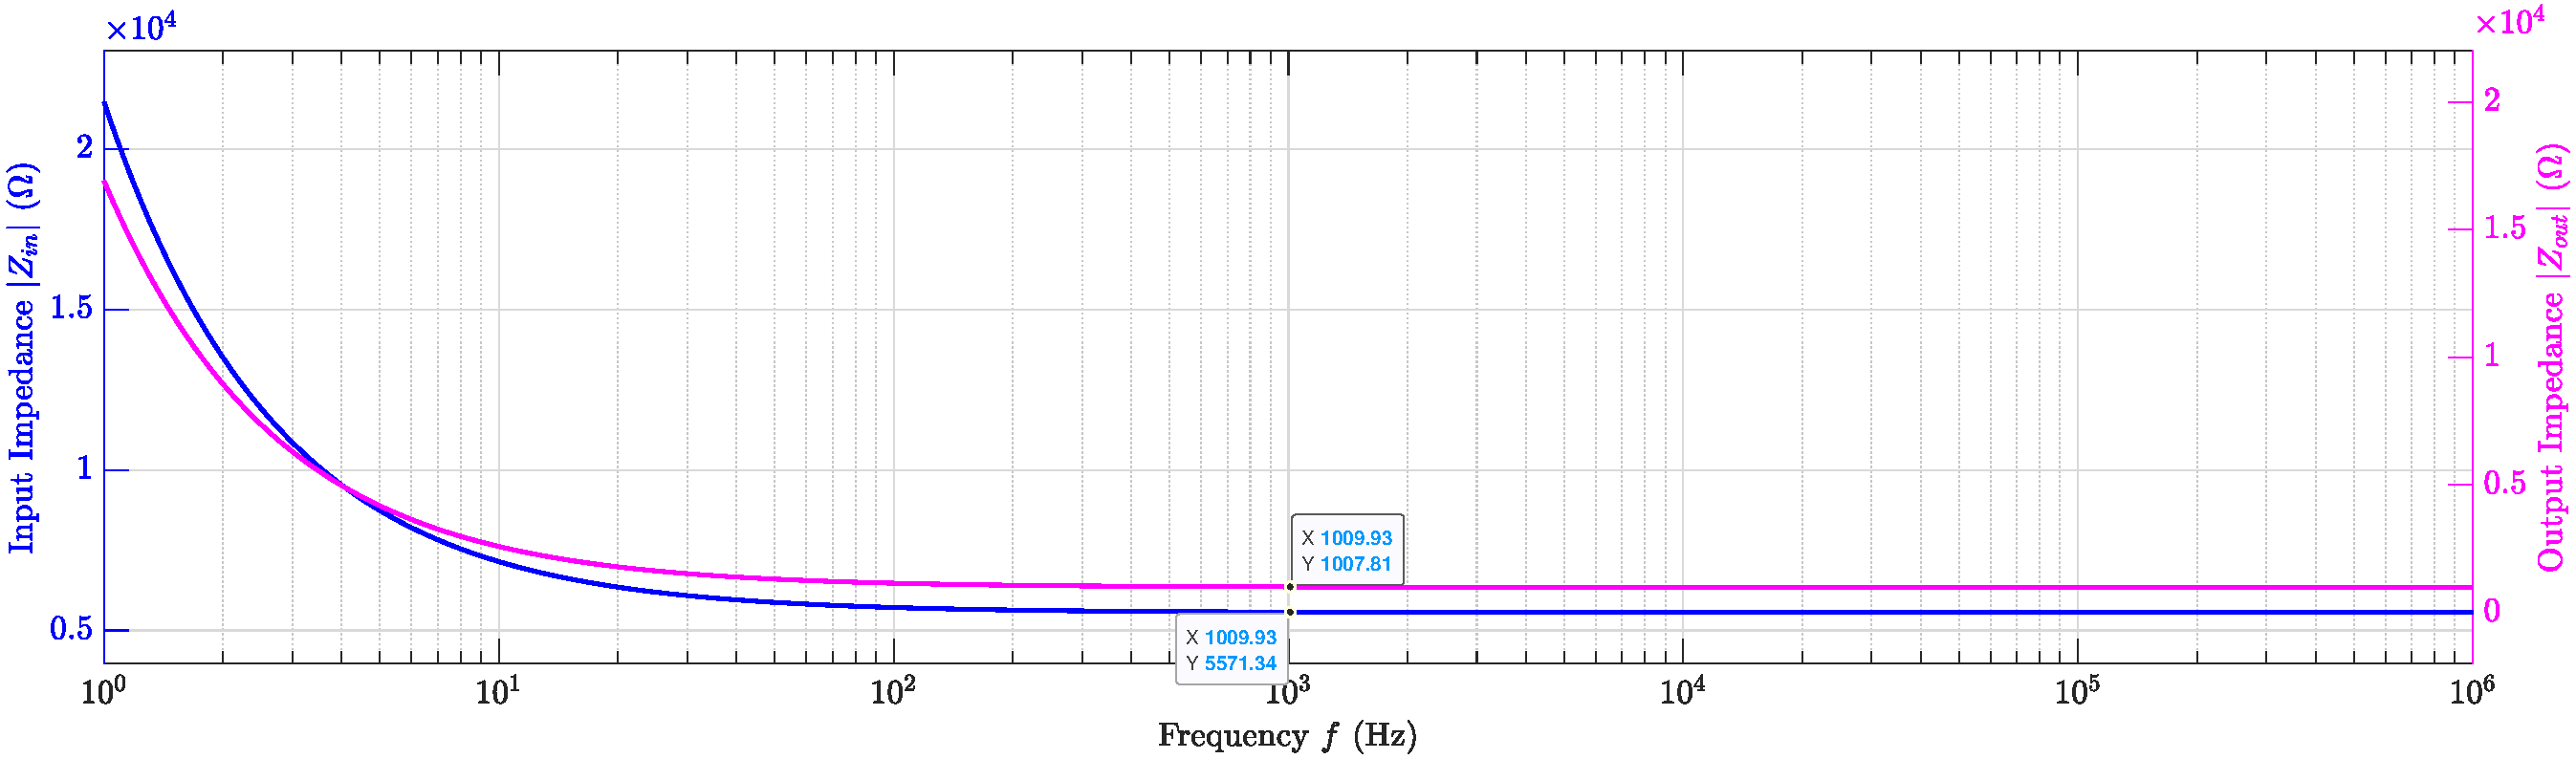
\includegraphics[width=\columnwidth]{LCE-02-三极管/assets/输入输出阻抗理论结果.pdf}
    \caption{Input and output impedance: theoretical results, $R_{in} = 5.571 \ \mathrm{k}\Omega$ @1kHz, $R_{out} = 1.007 \ \mathrm{k}\Omega$ @1kHz} 
    \label{fig: Input and output impedance theoretical results}
\end{figure}

\subsubsection{扫频法测量频率特性}

调整输入信号幅度为 20 mVamp, 频率为 100 Hz to 25 MHz (25 MHz is the maximum output frequency of the function generator),得到频率响应曲线如下:
\begin{figure}[H]\centering
    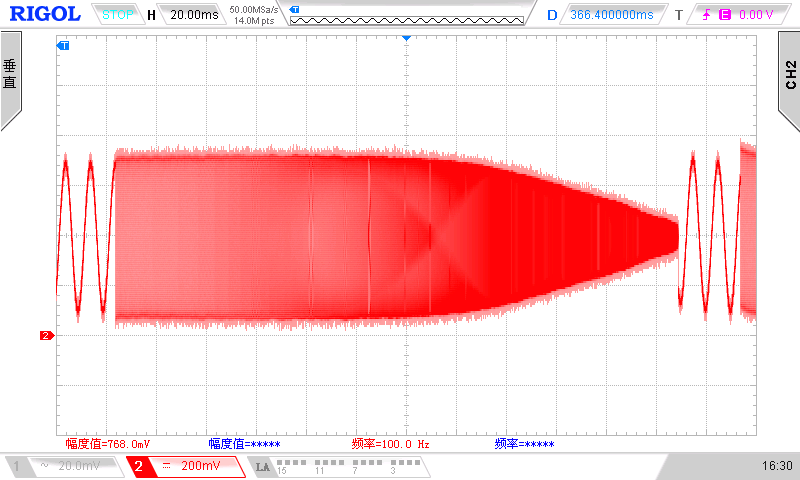
\includegraphics[width=\columnwidth]{LCE-02-三极管/assets/频率响应 100Hz to 25MHz.png}
    \caption{输出频率响应: input 20 mVamp (100 Hz $\sim$ 25 MHz), 输出电压 $V_{out}$ (CH2, red, dc coupling)}
\end{figure}
在原始中频增益下,输出电压峰峰值为 $634 \ \mathrm{mV}$,我们这里输入信号幅度没有变化,因此 -3dB 点对应的输出峰峰值为:
\begin{gather}
V_{out,pp}' = \frac{634 \ \mathrm{mV}}{\sqrt{2}} = 448.3057 \ \mathrm{mV} 
\end{gather}
在上面频率响应曲线中找到对应的峰峰值,展开后重新测量(这样采样率更高),得到截止频率约为:
\begin{gather}
f_c \approx 5.6 \ \mathrm{MHz}
\end{gather}

\begin{figure}[H]\centering
    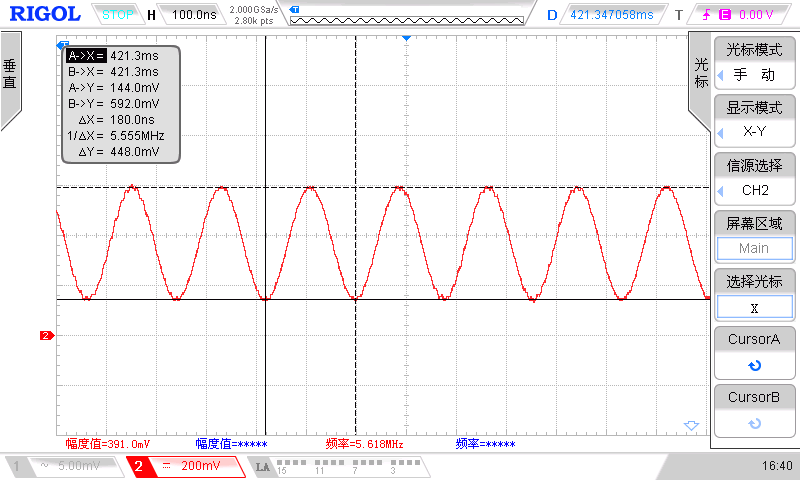
\includegraphics[width=\columnwidth]{LCE-02-三极管/assets/3dB 截止频率.png}
    \caption{CE 输出截止频率 $f_c$ :  input 20 mVamp, 输出电压 $V_{out}$ (CH2, red, dc coupling)}
\end{figure}

\subsection{共集放大电路 (Common-Collector Amplifier)}

\subsubsection{中频小信号增益}

更改跳线,将电路改为共集 (CC, EF) 组态,测量输入输出信号,获得的波形如下:

\begin{figure}[H]\centering
    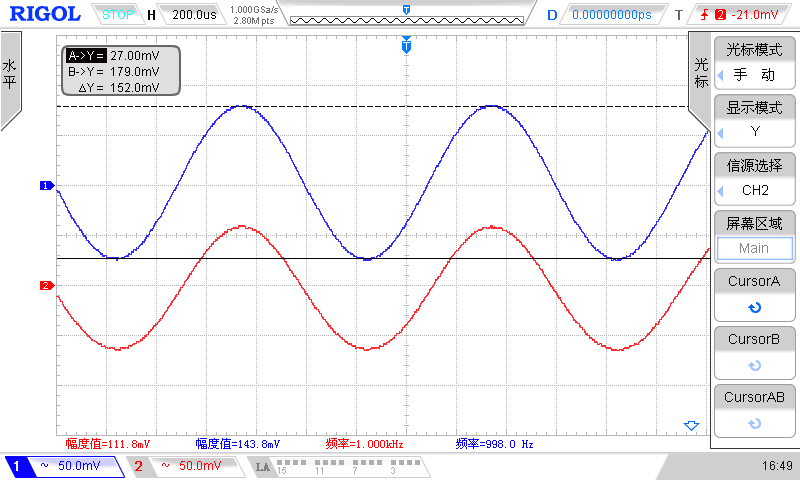
\includegraphics[width=\columnwidth]{LCE-02-三极管/assets/CC 输入 150 mV.png}
    \caption{CC amplifier I/O curve: input 150 mVamp, 有效输入 $V_{B}$ (CH1, blue),输出电压 $V_{out}$ (CH2, red),测量输入信号范围}
\end{figure}
\begin{figure}[H]\centering
    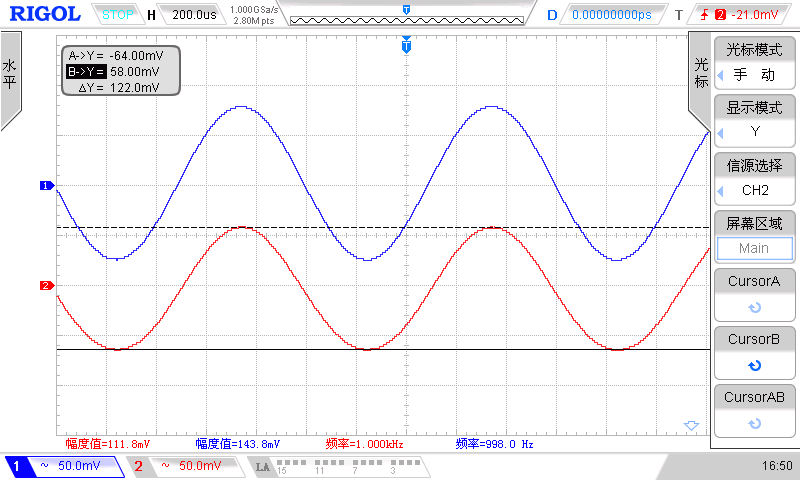
\includegraphics[width=\columnwidth]{LCE-02-三极管/assets/CC 输出 (约 122mV).png}
    \caption{CC amplifier I/O curve: input 150 mVamp, 有效输入 $V_{B}$ (CH1, blue),输出电压 $V_{out}$ (CH2, red),测量输出信号范围}
\end{figure}
依据图中数据,计算中频小信号增益 $A_0$:
\begin{gather}
A_0 = A_{v,1\mathrm{kHz}} = \frac{122 \ \mathrm{mV}}{152 \ \mathrm{mV}} = 0.8026
\end{gather}



\subsubsection{频率响应}

与前面类似,我们保持输入信号不变,将 $V_{out,pp}'$ 调整到 $ \frac{V_{out,pp}}{\sqrt{2}}$ 处,以获得 -3dB 截止频率。
\begin{gather}
    V_{out,pp}' = \frac{V_{out,pp}}{\sqrt{2}} = \frac{122 \ \mathrm{mV}}{\sqrt{2}} = 86.2670 \ \mathrm{mV}
    \Longrightarrow 
    f_c \approx 25 \ \mathrm{MHz}
\end{gather}

\begin{figure}[H]\centering
    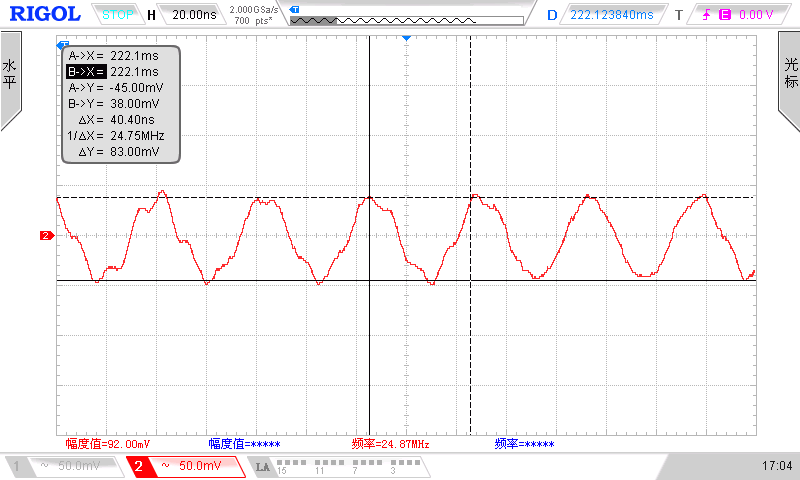
\includegraphics[width=\columnwidth]{LCE-02-三极管/assets/CC 3dB 截止频率.png}
    \caption{CC (EF) 输出截止频率 $f_c$ :  input 150 mVamp, 输出电压 $V_{out}$ (CH2, red, dc coupling)}
\end{figure}

\subsection{三极管的开关特性 (选做)}

% 断开 J1, J4, J5, 用杜邦线短路 $R_{E1}$ 和 $R_{E2}$ (J2, J3 随意) 使 emitter 接地, $R_{P1}$ 调至 100 kOhm (向断路靠近), base 作为输入端,有:
搭建如下图所示的三极管开关电路。检测完毕后接入开关信号(输入信号为加入直流偏置的方波,可以模拟开关信号),所得波形如图 \ref{fig: Switching circuit} 所示。

\begin{figure}[H]\centering
    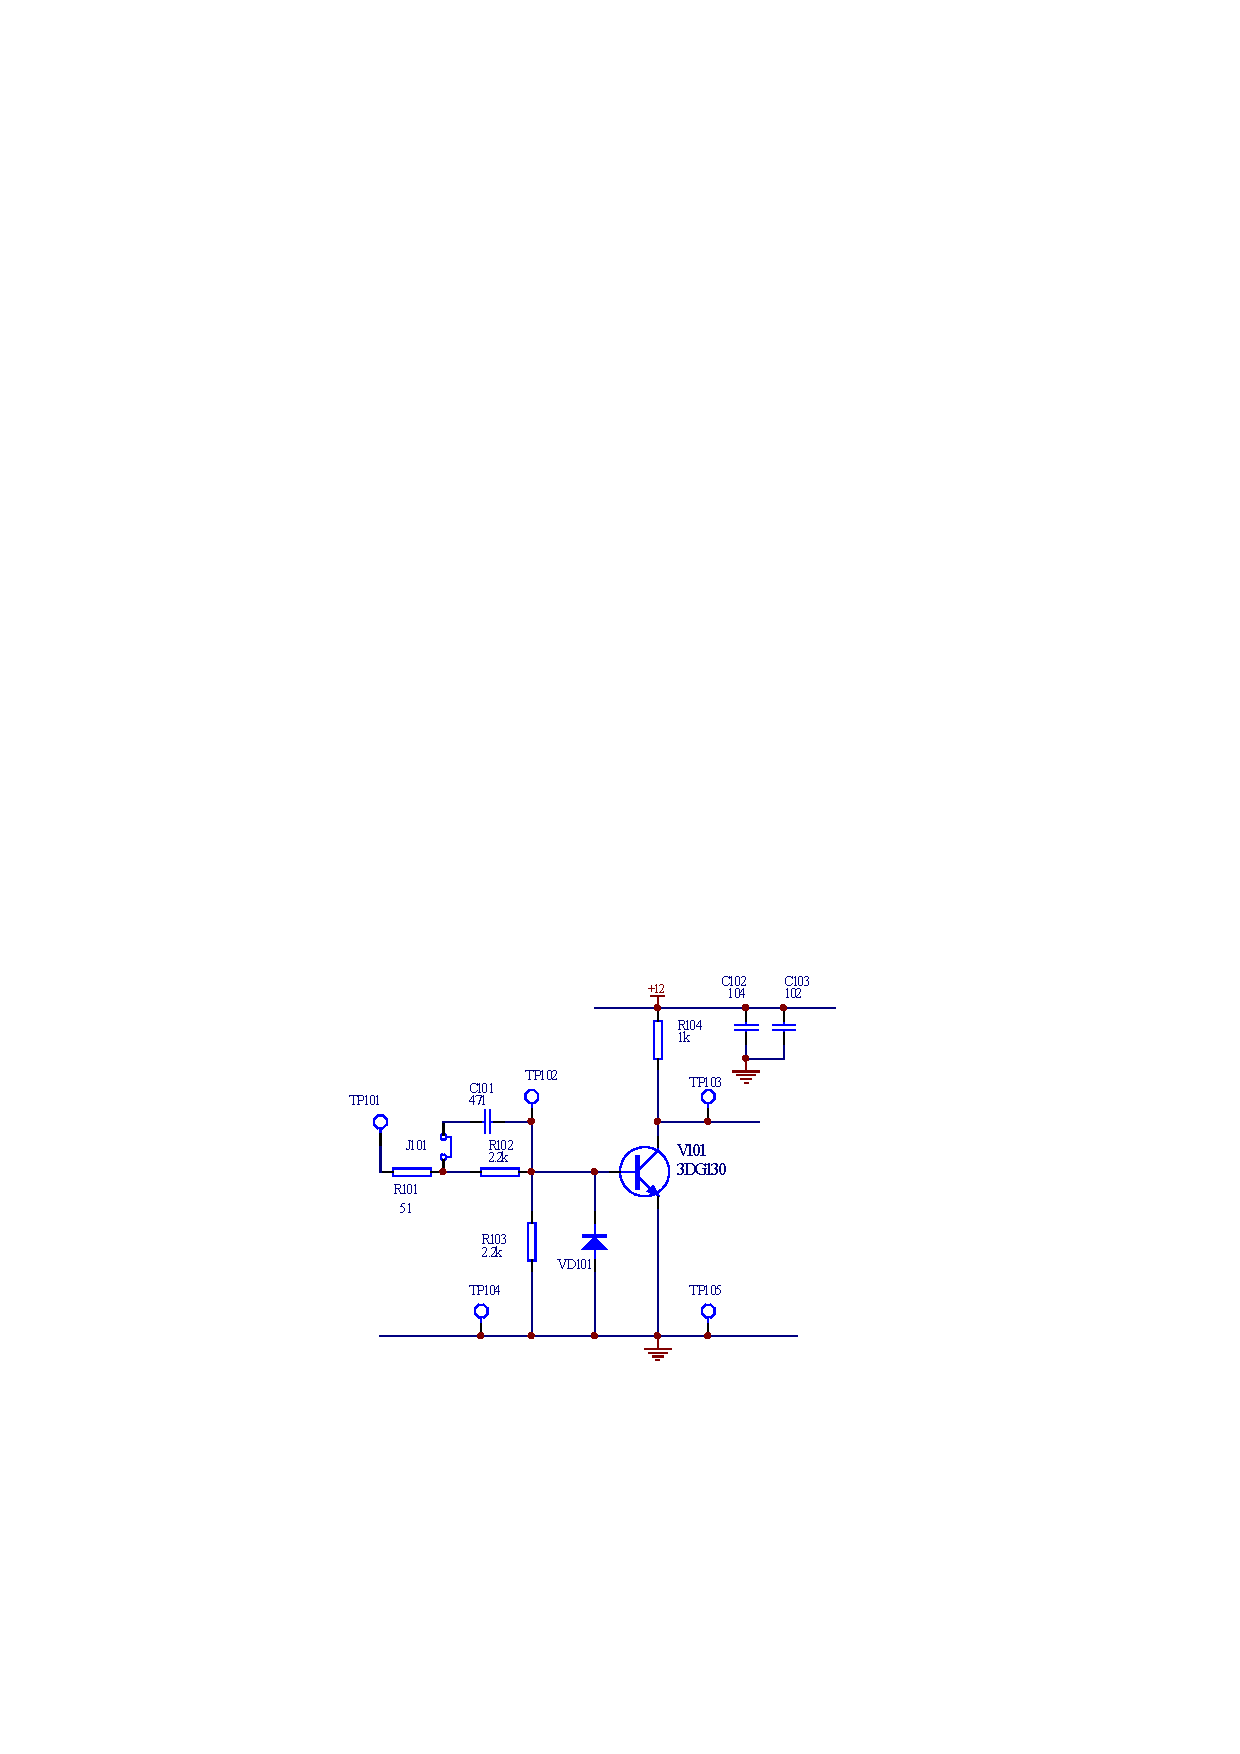
\includegraphics[width=0.5\columnwidth]{LCE-02-三极管/assets/开关电路电路图.pdf}
    \caption{三极管开关电路原理图}
\end{figure}

\begin{figure}[H]\centering
    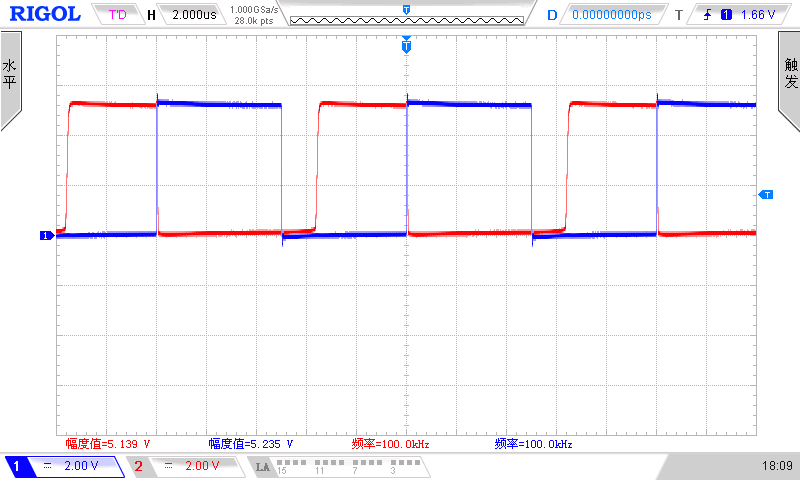
\includegraphics[width=\columnwidth]{LCE-02-三极管/assets/开关电路 无加速电容, input 100 kHz.png}
    \caption{Switching circuit: 无加速电容, input [0, 5V] square wave, 输入电压 $V_{in}$ (CH1, blue),输出电压 $V_{out}$ (CH2, red)}
    \label{fig: Switching circuit}
\end{figure}

\begin{figure}[H]\centering
    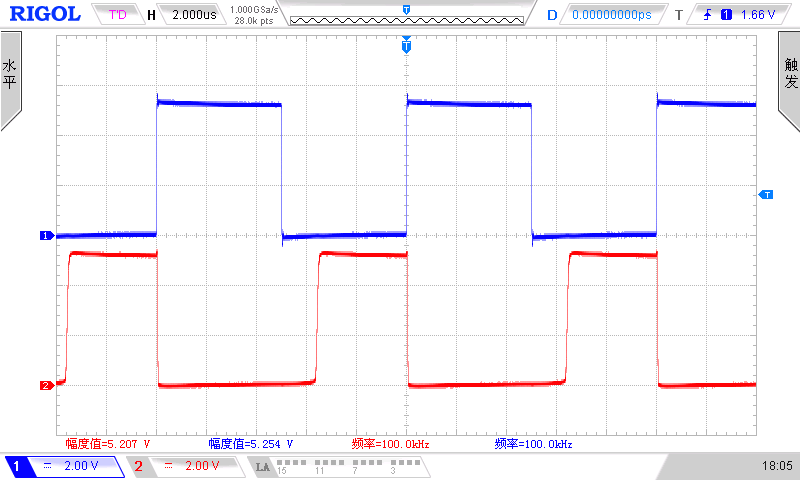
\includegraphics[width=\columnwidth]{LCE-02-三极管/assets/开关电路 无加速电容 (错位), input 100 kHz.png}
    \caption{Switching circuit: 无加速电容,  input [0, 5V] square wave, 输入电压 $V_{in}$ (CH1, blue),输出电压 $V_{out}$ (CH2, red), 错位}
\end{figure}

没有加速电容时,电路的延迟十分明显(在 us 量级),并入加速电容后,延迟时间明显降低(在几 ns 量级),如下图所示:

\begin{figure}[H]\centering
    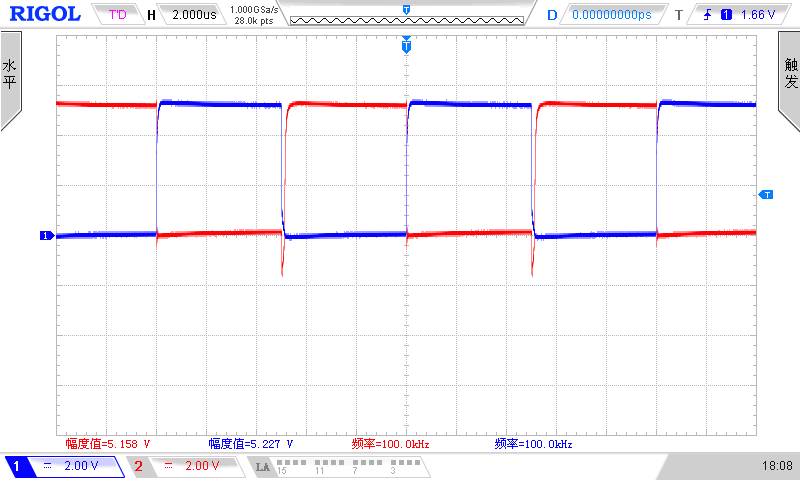
\includegraphics[width=\columnwidth]{LCE-02-三极管/assets/开关电路 有加速电容, input 100 kHz.png}
    \caption{Switching circuit: 有加速电容, input [0, 5V] square wave, 输入电压 $V_{in}$ (CH1, blue),输出电压 $V_{out}$ (CH2, red)}
\end{figure}

\begin{figure}[H]\centering
    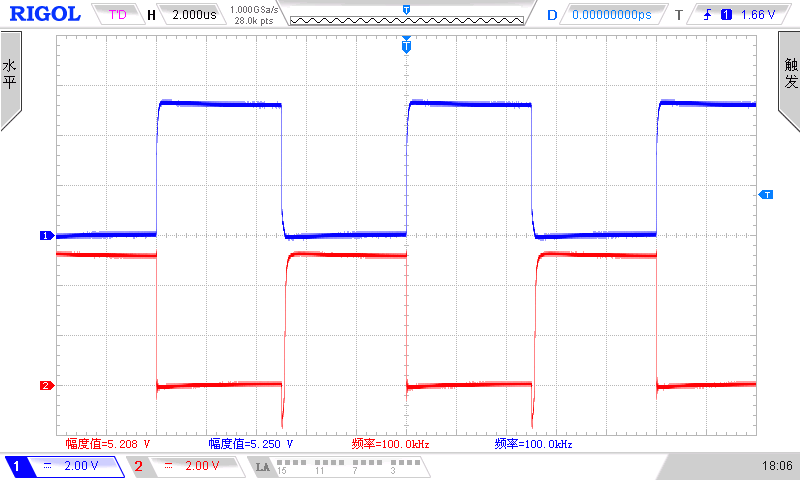
\includegraphics[width=\columnwidth]{LCE-02-三极管/assets/开关电路 有加速电容 (错位), input 100 kHz.png}
    \caption{Switching circuit: 有加速电容,  input [0, 5V] square wave, 输入电压 $V_{in}$ (CH1, blue),输出电压 $V_{out}$ (CH2, red), 错位}
\end{figure}

\newpage
\subsection{共基放大电路 (Common-Base Amplifier) (选做)}
通过更改跳线,将电路改为共基组态,观察输入输出信号增益和相位关系,获得的波形如下:
\begin{figure}[H]\centering
    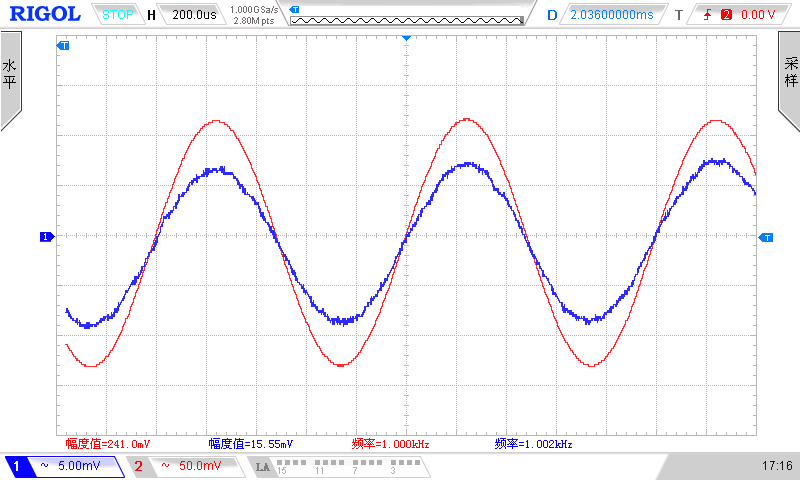
\includegraphics[width=\columnwidth]{LCE-02-三极管/assets/CB 输入输出.png}
    \caption{CB amplifier I/O curve: ac coupling, input 20 mVamp, 有效输入 $V_{B}$ (CH1, blue),输出电压 $V_{out}$ (CH2, red)}
\end{figure}
\begin{figure}[H]\centering
    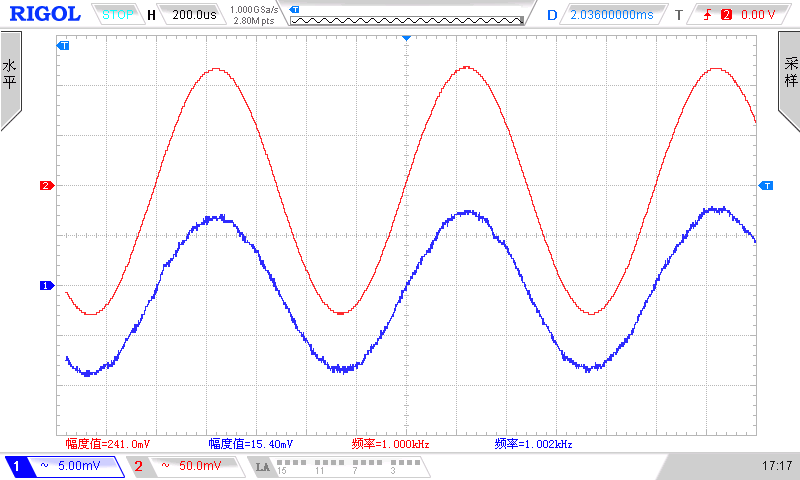
\includegraphics[width=\columnwidth]{LCE-02-三极管/assets/CB 输入输出 (错位).png}
    \caption{CB amplifier I/O curve: ac coupling, input 20 mVamp, 有效输入 $V_{B}$ (CH1, blue),输出电压 $V_{out}$ (CH2, red), 错位显示}
\end{figure}
















\section{思考题}

\subsection{共基极电路 (Common-Base Amplifier) 有哪些优缺点,你知道有哪些应用?}

优点:频率响应比共射组态更好,截止频率更高;缺点:输入阻抗小。常用于高频电路的小信号放大。

\subsection{单管共发射极电路,为获得最大输出幅度输出,静态工作点如何设置?}

静态工作点应使 $V_{C}$ (集电极电位) 约为 $\frac{V_{CC} - V_{CE,sat}}{2}$,以获得较平均的上下半输出,即为最大输出幅度。

\subsection{实验中,饱和失真出现很明显,截止失真波形则不明显,试分析原因}

饱和失真出现时,$\beta$ 急剧下降,导致小信号增益迅速跌落至(接近)零,因此饱和失真很明显;而截止失真是由于三极管的非线性特性造成的,电流 $I_C$ 下降时,小信号增益(近似)遵循二次根号下降,逐渐变小,也就是 $A_v \propto \sqrt{I_C}$,因此截止失真不明显。

\subsection{共射电路,为满足低频特性,电路中的三个电容,哪个容量最大?为什么?}

不妨对 common-emitter amplifier 的频率响应作详细分析,结论如下:

\begin{figure}[H]\centering
    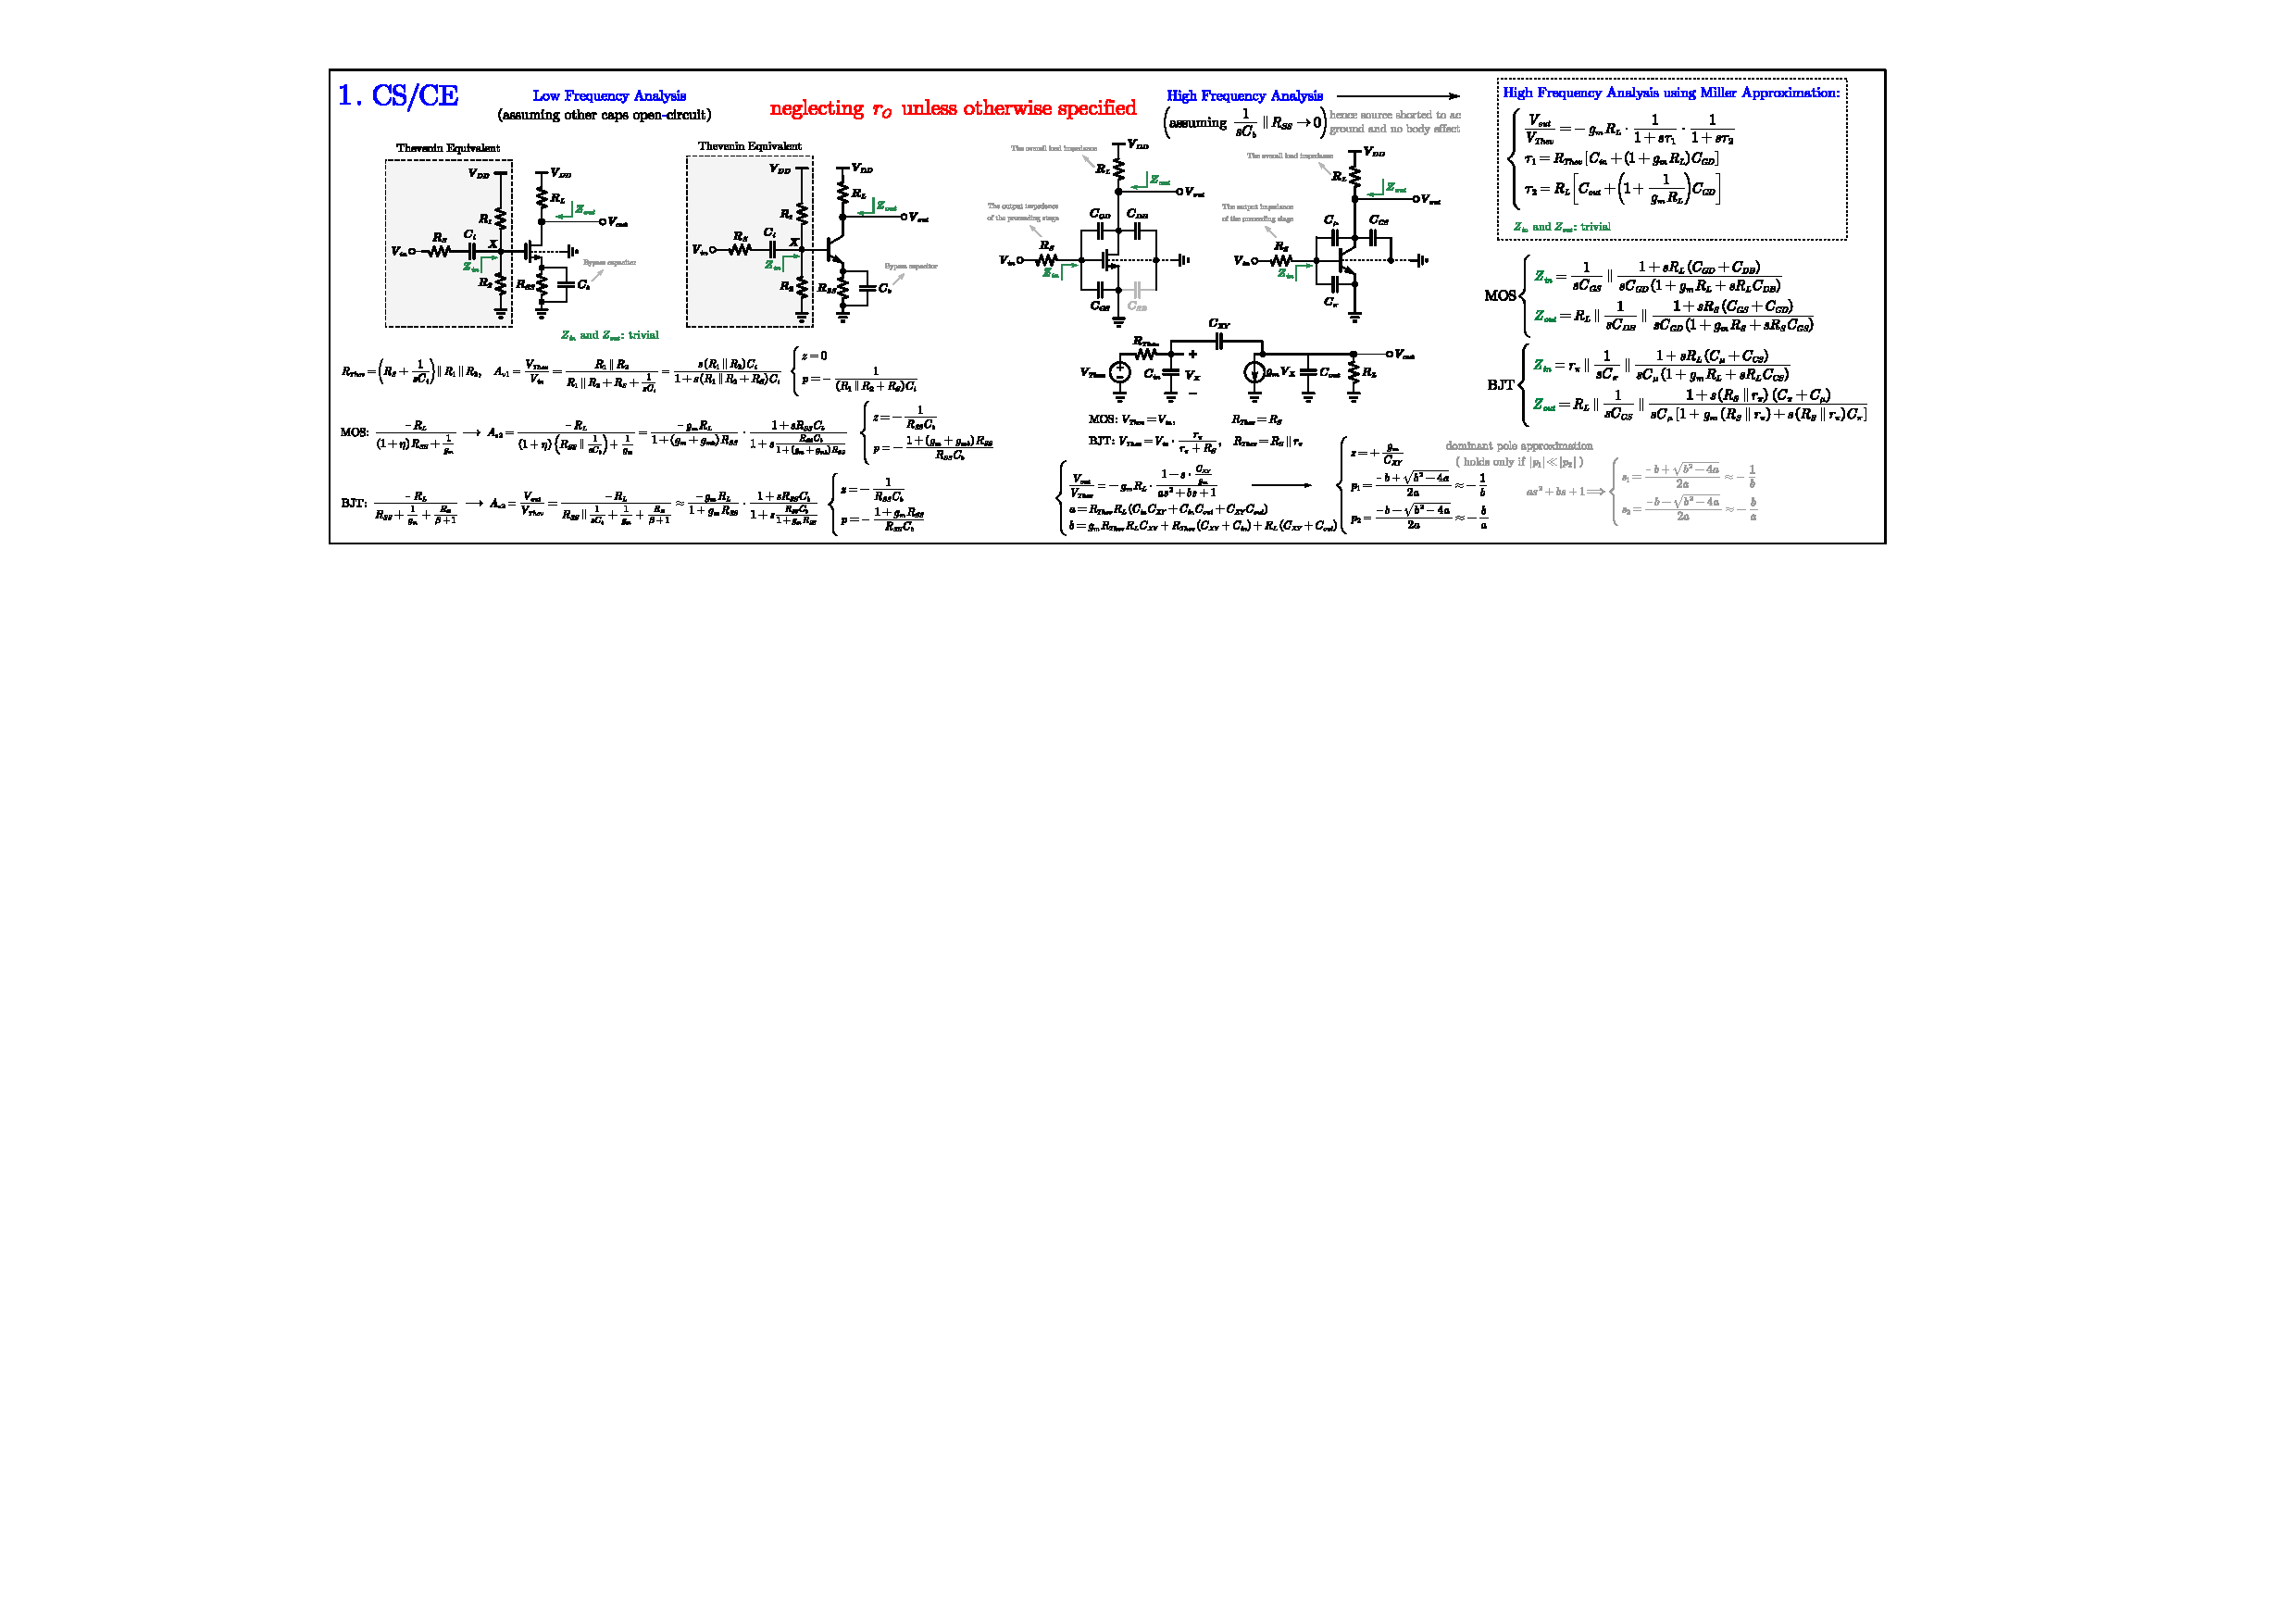
\includegraphics[width=\columnwidth]{LCE-02-三极管/assets/frequency analysis of CE.pdf}
    \caption{Frequency response of common-emitter amplifier}
\end{figure}

\noindent 影响低频增益的主要是零点位置,三个电容分别带来的零点分别为:
\begin{gather}
z_{C_{in}} = z_{C_{out}} = 0,\quad 
z_{C_{b}} = \frac{1}{R_{SS} C_b}
\end{gather}
零点频率越低,增益越早爬升到 midband gain, 因此要尽量提高 $C_{b}$ 的容量。$C_b$ 容量越大,低频增益越大(但过大会使 $C_b$ 的谐振频率过低,可能影响高频增益)。





\subsection{共射电路,高频截止频率约 1 MHz 左右,受制于什么?如何提高此频率?}

我们并没有完全按课件上的电路参数来做,实际测得的高频截止频率 (-3dB) 约 5.6 MHz。
在上一个思考题,我们已经对 common-emitter amplifier 的频率响应作了详细分析。继续应用上面的结论可以知道,这主要是由晶体管 base 和 collector 之间的寄生电容 $C_{\mu}$ (也写作 $C_{BC}$) 造成的,因为第一主极点为:
\begin{gather}
p_1 \approx \frac{1}{b} = \frac{1}{g_m (R_S \parallel r_{\pi}) R_C C_{\mu} + (R_S \parallel r_{\pi}) (C_{\mu} + C_{\pi}) + R_C (C_{\mu} + C_{CS})}
\approx 
\frac{1}{g_m (R_S \parallel r_{\pi}) R_C C_{\mu}}
\end{gather}
而第二主极点 $p_2 = \frac{b}{a} \gg p_1$,对高频截止频率影响不大。


\newpage
\section{实验建议}

\noindent 以下是对本次实验的一些建议:

\subsection{建议添加理论分析}

本次实验,共射放大电路是重点,对此电路的实验内容也很详尽。但美中不足的是,整个实验几乎没有任何定量的理论分析。截至上周,我们已经完成了晶体管及其放大电路的学习,除了与频响有关的问题,大多数同学可能无法回答,其它的内容已经完全可以进行定量的理论计算。包括但不限于“不出现饱和、截止失真时的最大输入输出范围”、“放大电路的中频小信号增益”、“放大电路的输入输出阻抗”。

在本次实验开始前,我自己对预习报告中涉及的共射极放大电路作了详细的实验,包括理论分析、仿真分析和实际电路验证,详见\textbf{附录 C (Experiment Report of Common Emitter Amplifier)}。

因此,希望从下一届同学开始,预习报告中应有适当的理论分析,让同学们感受理论预测与实测结果的区别,而不是仅仅记录了实验结果,却不明白背后的理论原理。

\subsection{频响思考题应给出参考理论}

思考题中有两题涉及到频响响应分析,由于“三极管的高频模型”和“电路的频响分析”,这两部分内容在线电课上还没有学,大多数同学不能很好地分析放大电路的频率响应和零极点,也就难以准确地、定量的回答“电容容量”和“高频截止频率”两个思考题。所以,如果能给出一些用于参考的理论分析,便可以辅助没有接触过频响内容的同学回答相关思考题,并从中学到知识。

\subsection{实验所用教材}

关于实验所用的参考教材《电子电路测量与设计实验 (第 2 版) (陈凌霄,孙丹丹,张晓磊,高英 编著)》,希望老师能把参考教材(的电子版)发给学生,否则,版本可能不同,预习要求中的对应页码(或内容顺序)会有偏差,找不到对应位置。例如,我自己在预习时,便没有能找到“按教材P173 图 6.1.8 电路确定元件参数”,我所用的电子版教材中,图 6.1.8 是 “在 Altium Designer19 的 Preference 对话框中设置纸张大小”。





%\section{异常现象分析}




















































% 附录 A
\newpage
\vspace*{\fill}\begin{center}\Huge{\bfseries 
    附录 A\hspace*{20pt} 预习报告
}\end{center}\addcontentsline{toc}{section}{附录 A\hspace*{6pt} 预习报告} 
\begin{figure}[H]\centering
    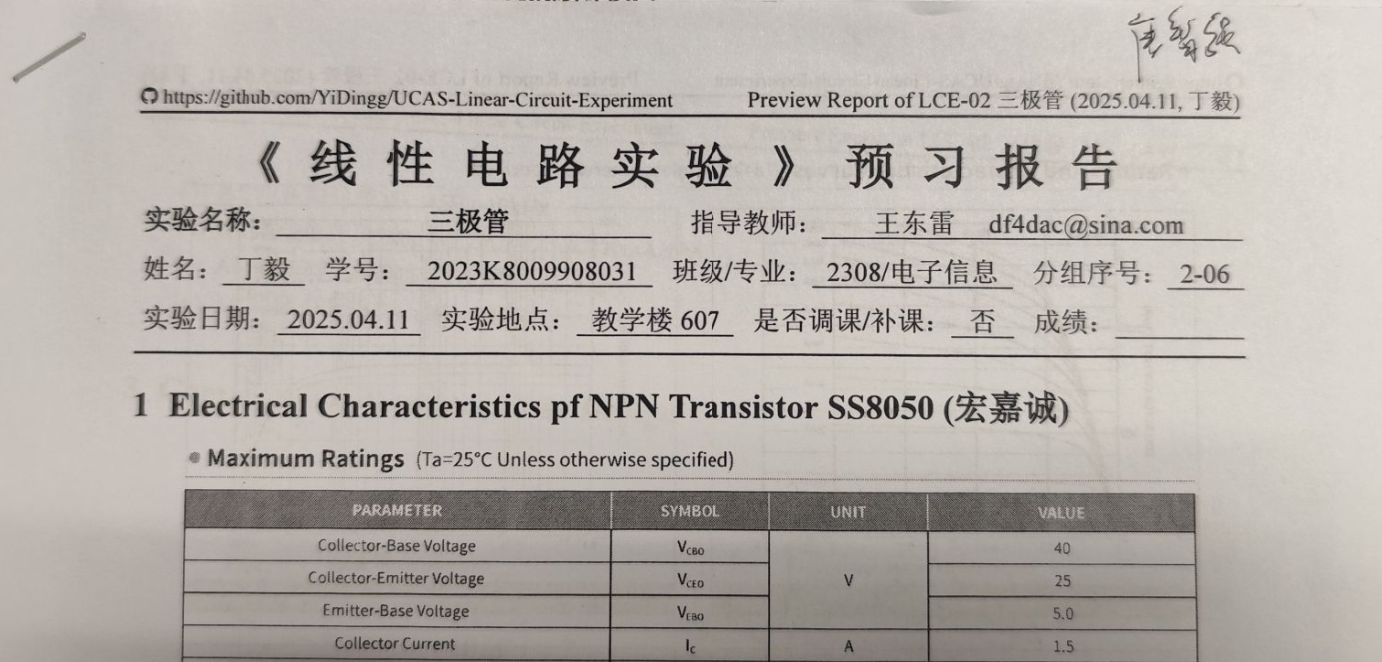
\includegraphics[width=\columnwidth]{LCE-02-三极管/assets/附录/预习报告.png}
\end{figure}
\vspace*{\fill}


\thispagestyle{fancy} 
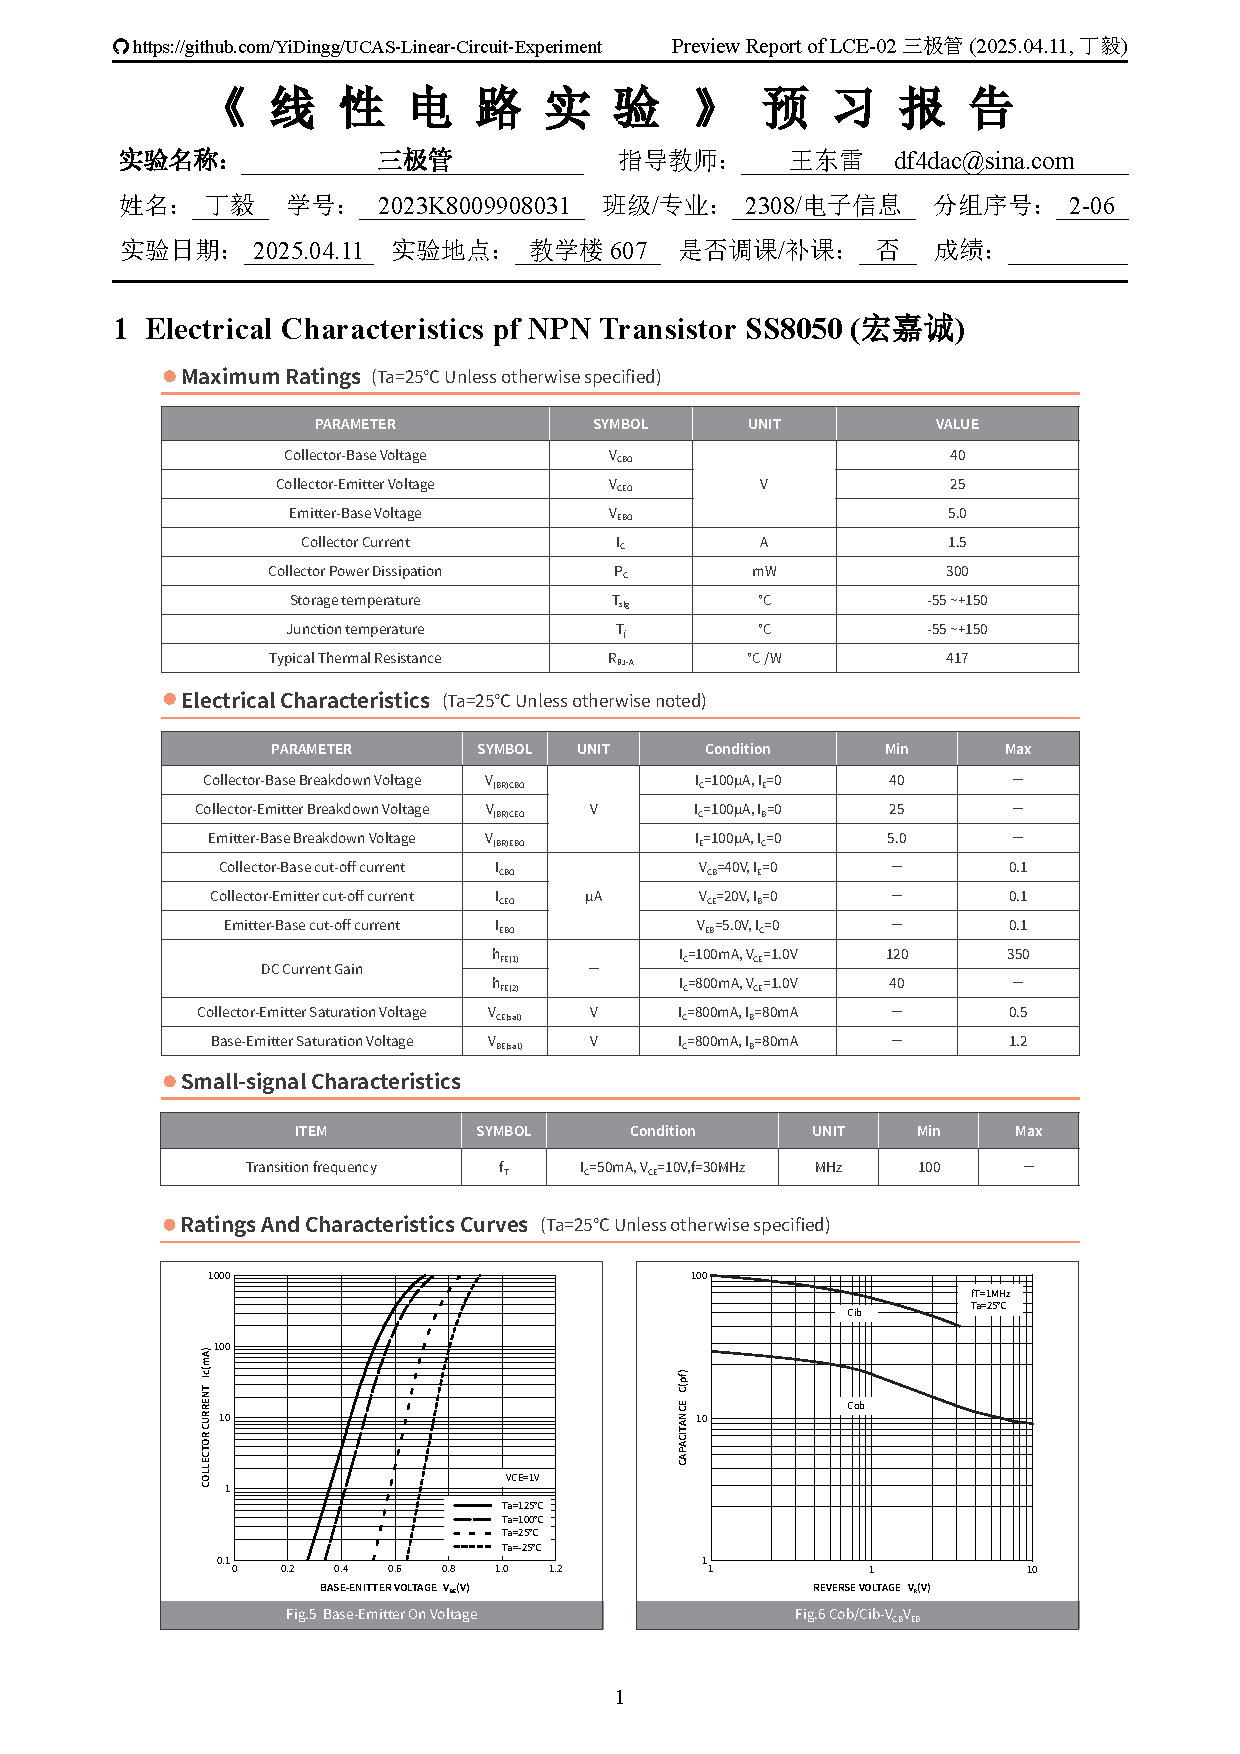
\includepdf[pages={-}]{LCE-02-三极管/preview/LCE-02 (preview report).pdf}

% 附录 B
\newpage
\begin{center}\Huge{\bfseries 
    附录 B\hspace*{20pt} 原始数据记录表
}\end{center}
\addcontentsline{toc}{section}{附录 B\hspace*{6pt} 原始数据记录表} 
\thispagestyle{fancy} 
\begin{figure}[H]\centering
    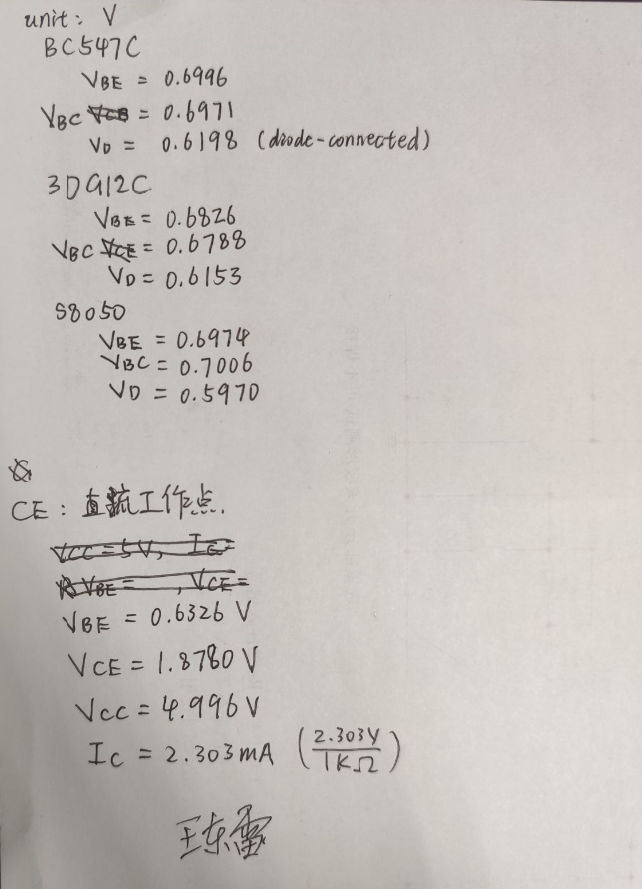
\includegraphics[width=0.9\columnwidth]{LCE-02-三极管/assets/附录/原始数据.png}
\end{figure}


% 附录
\newpage
\vspace*{\fill}\begin{center}\Huge{\bfseries 
    附录 C \hspace*{20pt} Experiment Report of Common Emitter Amplifier
}\end{center}\vspace*{\fill}
\addcontentsline{toc}{section}{附录 C \hspace*{6pt} Experiment Report of Common Emitter Amplifier}
\thispagestyle{fancy} 
\includepdf[page=-]{LCE-02-三极管/assets/Common Emitter Amplifier Experiment.pdf}



\end{document}

% VScode 常用快捷键:

% F2:                       变量重命名
% Ctrl + Enter:             行中换行
% Alt + up/down:            上下移行
% 鼠标中键 + 移动:           快速多光标
% Shift + Alt + up/down:    上下复制
% Ctrl + left/right:        左右跳单词
% Ctrl + Backspace/Delete:  左右删单词    
% Shift + Delete:           删除此行
% Ctrl + J:                 打开 VScode 下栏(输出栏)
% Ctrl + B:                 打开 VScode 左栏(目录栏)
% Ctrl + `:                 打开 VScode 终端栏
% Ctrl + 0:                 定位文件
% Ctrl + Tab:               切换已打开的文件(切标签)
% Ctrl + Shift + P:         打开全局命令(设置)

% Latex 常用快捷键:

% Ctrl + Alt + J:           由代码定位到PDF


